%% Manuscript for Chaos (AIP Publishing), prepared with the official AIP template
%% (REVTeX 4.1 with the AIP substyles, files included in this directory).
%% Compile: pdflatex main && bibtex main && pdflatex main && pdflatex main
%% For the peer-review format required by AIP, replace "reprint" by "preprint".
\documentclass[%
 aip,
 cha,
 amsmath,amssymb,
 reprint,%
 longbibliography,%
]{revtex4-1}

\usepackage{graphicx}% Include figure files
\usepackage{dcolumn}% Align table columns on decimal point
\usepackage{bm}% bold math
\usepackage[utf8]{inputenc}
\usepackage[T1]{fontenc}
\usepackage{mathptmx}
\usepackage{etoolbox}
\usepackage[hidelinks]{hyperref}

%% Apr 2021: AIP requests that the corresponding
%% email to be moved after the affiliations
\makeatletter
\def\@email#1#2{%
 \endgroup
 \patchcmd{\titleblock@produce}
  {\frontmatter@RRAPformat}
  {\frontmatter@RRAPformat{\produce@RRAP{*#1\href{mailto:#2}{#2}}}\frontmatter@RRAPformat}
  {}{}
}%
\makeatother

% float placement: several full-width figures
\renewcommand{\topfraction}{0.92}
\renewcommand{\bottomfraction}{0.8}
\renewcommand{\textfraction}{0.06}
\renewcommand{\floatpagefraction}{0.75}
\renewcommand{\dbltopfraction}{0.95}
\renewcommand{\dblfloatpagefraction}{0.75}
\setcounter{topnumber}{3}
\setcounter{dbltopnumber}{3}
\setcounter{totalnumber}{5}

% \PIARlayout{<preprint>}{<reprint>}: selects a layout setting according to the class
% option, so that the article formats acceptably under preprint (the AIP review format)
\makeatletter
\newcommand{\PIARlayout}[2]{\preprintsty@sw{#1}{#2}}
\makeatother
% REVTeX sets \sloppy in two-column mode; the same line breaking is used in preprint mode
\AtBeginDocument{\PIARlayout{\sloppy}{}}

% Zenodo DOI of the code and data archive: fill in after reserving the DOI (e.g. 10.5281/zenodo.1234567)
\newcommand{\zenodoDOI}{}

\begin{document}

\preprint{AIP/CHAOS}

\title[From separatrix to strange attractor]{From separatrix to strange attractor: Physics-informed normalizing flows for recovering missing dynamics in a spring-coupled inverted pendulum}

\author{Fredy Alexander Orjuela L\'opez}
\email{fa.orjuela@uniandes.edu.co}
\affiliation{Departamento de F\'isica, Universidad de los Andes, Bogot\'a, Colombia}

\date{\today}

\begin{abstract}
Sensor records of mechanical systems are seldom complete, and the missing dynamics must be inferred. The full--partial reconstruction mapping (FPRM) uses Takens' embedding theorem to learn the map between the delay reconstructions of a complete and an incomplete signal. The FPRM is extended and tested on the spring-coupled inverted pendulum (PIAR), a minimal model of inverted-pendulum seismic isolators controlled by one parameter $\mu=kL/(Mg)-1$. Five canonical regimes, from a libration inside the upright well to rotations near and far from the separatrix, are characterized with closed-form invariants and trajectories conserving energy to $10^{-10}\,MgL$. Under damping and forcing, a Feigenbaum cascade leads to a strange attractor with largest Lyapunov exponent $0.096\,(g/L)^{1/2}$ and Kaplan--Yorke dimension $2.28$. A cross-mapping analysis shows that the reflection $\theta\to-\theta$ makes the spring-force sign unrecoverable from the collar height unless the forcing phase is known. To represent such ambiguity, the Gaussian-process engine of the FPRM is replaced by a conditional neural spline flow, optionally regularized by equation-of-motion residuals. With the spring force observed and $90\%$ of the collar-height and angular-velocity records missing, the physics-regularized flow lowers the continuous ranked probability score 4.5-fold relative to the original FPRM (threefold when its Gaussian process uses all labeled samples) and restores the fractal Poincar\'e section; for ambiguous targets, the unregularized flow preserves both branches, whereas residuals blind to the branch can induce mode collapse. An open laboratory, comprising a browser-based interactive simulation and a Python package that regenerates every figure and number, makes the PIAR a transparent benchmark for dynamics-informed reconstruction.
\end{abstract}


\maketitle

\begin{quotation}
An upright rod held by a spring seems a textbook exercise, yet the same principle shields gravitational-wave detectors from ground vibration: when the spring almost cancels gravity, the pendulum sways so slowly that seismic noise is filtered out. Monitoring such devices requires their full state, but sensor records are often incomplete. The full--partial reconstruction mapping is a recent machine-learning framework that fills the gaps by exploiting a classic result of nonlinear dynamics: the history of one measured signal encodes the geometry of the whole motion, from which a missing signal can be read off. The framework is tested here on the spring-coupled inverted pendulum, a system simple enough for every prediction to be checked against exact mechanics and rich enough to become chaotic when damped and driven. A mirror symmetry of the pendulum can make the missing signal ambiguous, and regression then averages two possible answers into an impossible one. A normalizing flow, a neural network that returns a full probability distribution, keeps both answers and recovers the chaotic motion when nine tenths of one sensor's readings are missing, whereas physical constraints imposed as soft penalties help with scarce data only where they can reliably tell the mirror states apart.
\end{quotation}


\section{Introduction}\label{sec:intro}

Inverted pendulums are among the most effective passive low-frequency mechanical filters. In the seismic attenuation chains of interferometric gravitational-wave detectors, rigid legs hold the payload in the unstable upright configuration while an elastic element is tuned to almost cancel the gravitational antispring, so that the resonance frequency falls far below the seismic band and ground motion is strongly suppressed~\cite{Losurdo1999,Takamori2007}. The spring-coupled inverted pendulum (PIAR, the acronym of its Spanish name, \textit{p\'endulo invertido acoplado a un resorte}) captures this principle in its simplest form: a rigid rod pivoted at its lower end carries a mass and is held upright by a horizontal spring whose far end rides on a collar that slides along a vertical guide. Its conservative dynamics is controlled by a single dimensionless number, $\mu=kL/(Mg)-1$, which measures how much the elastic restoring torque exceeds the gravitational toppling torque. As $\mu\to0^{+}$ the small-oscillation frequency vanishes, which is the property sought for isolation, but the energy barrier that protects the upright position vanishes even faster, which is its price. Once damping and periodic forcing are added, the same model displays, in its weak-spring regime ($\mu<0$), the period-doubling route to chaos familiar from the driven pendulum~\cite{BakerGollub1996,Strogatz2015,GuckenheimerHolmes1983}. Inverted pendulums also remain paradigmatic models of stability and of its dynamic control~\cite{Butikov2001}. Practical relevance, analytical tractability, and dynamical richness thus meet in a single degree of freedom.

Practical relevance, however, comes with a practical difficulty. The state of an isolator is rarely measured completely: angle sensors, load cells, and position encoders drop out, saturate, or are simply absent, and the unmeasured variables must be inferred from the measured ones. Statistics treats this situation as a missing-data problem~\cite{LittleRubin2019}, and deep imputation methods for time series, from bidirectional recurrent networks~\cite{Cao2018} to Gaussian-process variational autoencoders~\cite{Fortuin2020} and score-based diffusion models~\cite{Tashiro2021}, have become remarkably accurate on generic benchmarks. For deterministic, and in particular chaotic, dynamics a different and more physical route exists. Delay coordinates of a single observable reconstruct the attractor of the system~\cite{Packard1980,Takens1981}, generically and up to a smooth change of coordinates~\cite{Sauer1991}. Nonlinear time-series analysis and prediction~\cite{Abarbanel1993,KantzSchreiber2004,Casdagli1989,Pathak2018}, the detection of causality by cross mapping between reconstructed manifolds~\cite{Sugihara2012}, and the inference of unmeasured variables with reservoir computers~\cite{Lu2017} all rest on this fact, which has become a main point of contact between machine learning and complex systems~\cite{Tang2020}.

The full--partial reconstruction mapping (FPRM), recently introduced by Wu et al.~\cite{Wu2026FPRM}, turns this geometric fact into an imputation method. The delay reconstruction of a completely observed time series and that of a partially observed one are both faithful images of the same attractor; the map between them can therefore be learned at the times at which both series are available and evaluated wherever the partial series is missing. Implemented with Gaussian-process regression (GPR)~\cite{Rasmussen2006}, the FPRM recovers complex dynamics even when most of the data are missing, and it rests on a transparent justification rooted in dynamical-systems theory. Two questions left open by the original formulation become pressing for mechanical systems. The first concerns identifiability: Takens' theorem holds for generic observables, but physical symmetries can make a measured quantity nongeneric~\cite{LetellierAguirre2002,Letellier2005}. The missing value is then no longer a function of the delay coordinates, its conditional distribution becomes multimodal, and a Gaussian regressor returns the average of the branches, a value that the system never visits. The second question concerns physics: the equations of motion of a mechanical system are usually known, at least in form, and it is natural to ask whether imposing them improves the reconstruction.

Conditional generative models address the first question by construction. Normalizing flows~\cite{Papamakarios2021,Durkan2019}, variational autoencoders~\cite{Kingma2014,Sohn2015}, and denoising diffusion models~\cite{Ho2020,NicholDhariwal2021} learn full conditional distributions and can represent several branches at once. Physics-informed learning~\cite{Raissi2019,Karniadakis2021} addresses the second question by adding the residuals of known equations to the training loss. Structure-preserving architectures, such as Hamiltonian and Lagrangian neural networks~\cite{Greydanus2019,Cranmer2020} and symplectic networks~\cite{Jin2020}, instead build conservation laws into the model itself. Soft physical constraints are known, however, to reshape the loss landscape in ways that can impair training~\cite{Krishnapriyan2021,WangTengPerdikaris2021}, and whether they help a generative imputer is an open empirical question.

The PIAR is a well-suited test bed for both questions. Its invariants (equilibria, barrier, separatrix energies, and normal form) are available in closed form, and its periods as quadratures, so that numerical and learned results can be checked against exact mechanics. Its two natural measurements, the spring force and the height of the collar, are nontrivial functions of the angle that cannot be converted into each other by differentiation, and the reflection $\theta\to-\theta$ makes the first odd and the second even, which creates a controlled, physically motivated identifiability problem. Its bifurcation parameter provides a single axis along which the dynamics changes qualitatively, and, under forcing, the system develops a strange attractor of low and measurable dimension.

This article develops the PIAR into a benchmark for dynamics-informed reconstruction and uses it to extend the FPRM in three respects: a symmetry analysis, verified by a model-free cross-mapping test, that establishes in advance which reconstruction tasks are identifiable; a generative engine, a conditional normalizing flow, that represents the multimodal distributions that arise when identifiability fails; and a controlled assessment of when equation-of-motion residuals improve the reconstruction and when they induce mode collapse. Section~\ref{sec:model} presents the analytical mechanics in a self-contained form, and Sec.~\ref{sec:cases} uses high-accuracy integration and exact periods to characterize five canonical regimes of the conservative dynamics, which span the three stability classes of the upright position. Section~\ref{sec:chaos} follows the damped--driven dynamics through a Feigenbaum cascade to a strange attractor, uses Melnikov's method to locate the splitting of the separatrix from which chaos grows, and relates the dimension of the attractor to the embedding dimension required by Takens' theorem. Section~\ref{sec:fprm} establishes, by a model-free cross-mapping analysis, which reconstruction tasks are well posed and how the phase of the forcing restores the identifiability broken by the reflection symmetry; on this basis, the Gaussian-process engine of the FPRM is replaced by a conditional neural spline flow, optionally regularized by equation-of-motion residuals. Section~\ref{sec:results} benchmarks the resulting generative FPRM against the original method and against variational and diffusion alternatives. Section~\ref{sec:lab} describes the open, interactive laboratory that regenerates every figure and number of this article from fixed random seeds, Sec.~\ref{sec:discussion} discusses the implications and limitations of the results, and Sec.~\ref{sec:conclusions} summarizes the conclusions.

\section{The spring-coupled inverted pendulum}\label{sec:model}

\begin{figure*}
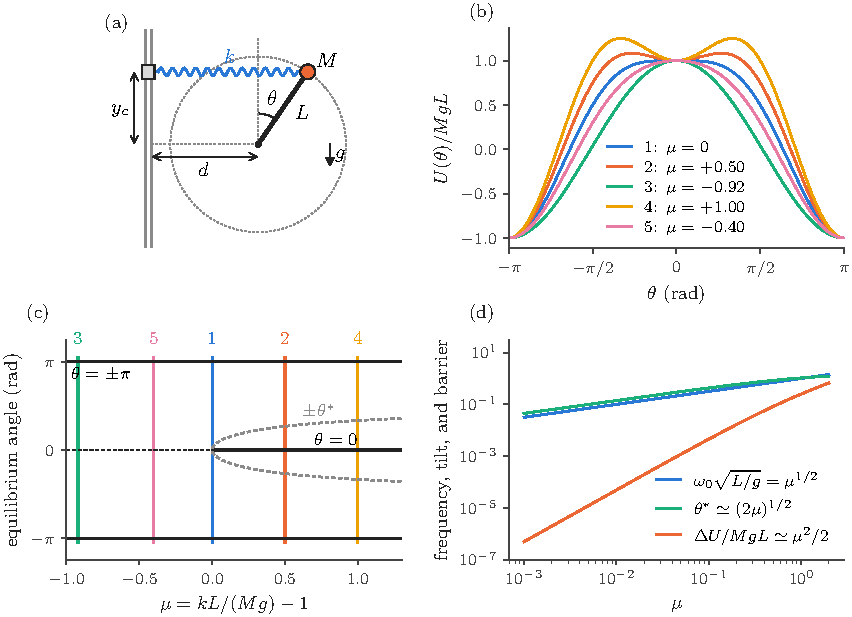
\includegraphics[width=\textwidth]{figures/fig_model.pdf}
\caption{Model and bifurcation. (a) Schematic of the PIAR: massless rod of length $L$ with a point mass $M$, and horizontal spring of stiffness $k$ attached to a collar that slides along a vertical guide, at a distance $d>L$ from the pivot, following the height $y_c=L\cos\theta$ of the mass; the elongation of the spring equals $L\sin\theta$, and the dashed circle is the path of the mass. (b) Potential energy, Eq.~\eqref{eq:U}, in units of $MgL$ for the values of $\mu$ of the five cases of Sec.~\ref{sec:cases}. (c) Equilibrium angles versus $\mu$, showing the subcritical pitchfork at $\mu=0$ (solid lines, stable; dashed lines, unstable); colored vertical lines mark the five cases. (d) Scales that vanish at the critical point: small-oscillation frequency, Eq.~\eqref{eq:omega0}; tilt of the saddles, Eq.~\eqref{eq:thetastar}; and barrier height, Eq.~\eqref{eq:barrier}.}
\label{fig:model}
\end{figure*}

\subsection{Geometry and measurable observables}\label{sec:geometry}

The PIAR is sketched in Fig.~\ref{fig:model}(a). A massless rigid rod of length $L$ pivots without friction about its lower end and carries a point mass $M$ at its upper end. The angle $\theta$ is measured from the upward vertical, so that $\theta=0$ is the upright position and $\theta=\pi$ the hanging one. A spring of stiffness $k$ joins the mass to a massless collar that slides freely along a vertical guide placed at a distance $d>L$ from the pivot, so that the mass can pass between the guide and the pivot during a full revolution. Because the collar follows the height of the mass, the spring remains horizontal, and, when its natural length equals $d$, its elongation is exactly the horizontal displacement of the mass, $L\sin\theta$: the spring is stretched when the mass moves away from the guide and compressed when it moves toward it. Two quantities of this arrangement can be measured without access to the angle itself, and both play a central role in the reconstruction problem of Sec.~\ref{sec:fprm}. The first is the spring force (the tension of the spring, positive in extension),
\begin{equation}
F_s = kL\sin\theta ,
\label{eq:Fs}
\end{equation}
which a load cell in series with the spring records; the second is the height of the collar above the pivot,
\begin{equation}
y_c = L\cos\theta ,
\label{eq:yc}
\end{equation}
which a linear encoder on the guide records. After calibration, the normalized channels $s=F_s/(kL)=\sin\theta$ and $c=y_c/L=\cos\theta$ are used throughout. Together they are the two coordinates of the mass on a unit circle and determine the angle, but each of them alone determines it only up to a reflection: $s$ is unchanged by $\theta\to\pi-\theta$, which exchanges the upper and lower half-planes, and $c$ by $\theta\to-\theta$, which exchanges the left and right half-planes.

\subsection{Energies and equation of motion}\label{sec:lagrangian}

The mass moves on a circle of radius $L$ about the pivot, so that its kinetic energy is that of a point mass with moment of inertia $ML^{2}$,
\begin{equation}
K = \tfrac12 ML^{2}\dot\theta^{2},
\label{eq:K}
\end{equation}
where the dot denotes a derivative with respect to time $t$. The potential energy contains a gravitational contribution, due to the height $L\cos\theta$ of the mass, and an elastic contribution, due to the elongation $L\sin\theta$ of the spring,
\begin{equation}
U(\theta) = MgL\cos\theta + \tfrac12 kL^{2}\sin^{2}\theta ,
\label{eq:U}
\end{equation}
with $g$ the gravitational acceleration. The two terms compete: gravity lowers the energy when the rod tilts away from the vertical, whereas the spring raises it. The Lagrangian $\mathcal L=K-U$ and the Euler--Lagrange equation, $\mathrm d(\partial\mathcal L/\partial\dot\theta)/\mathrm dt=\partial\mathcal L/\partial\theta$~\cite{Goldstein2002}, yield the equation of motion
\begin{equation}
ML^{2}\ddot\theta = MgL\sin\theta - kL^{2}\sin\theta\cos\theta ,
\label{eq:torque}
\end{equation}
which is the balance of torques about the pivot. The first term on the right-hand side is the gravitational torque, which tips the rod away from the vertical; the second is the torque of the restoring force that the spring exerts on the mass, $-F_s$, applied at the height $L\cos\theta$, which pulls the rod back toward the vertical while the mass is above the pivot. Dividing by the moment of inertia gives the standard form
\begin{equation}
\ddot\theta + \lambda\sin\theta\cos\theta - \beta\sin\theta = 0,
\qquad \lambda = \frac{k}{M},\quad \beta = \frac{g}{L},
\label{eq:eom}
\end{equation}
in which $\lambda$ and $\beta$ are the squared angular frequencies associated with the spring and with gravity, respectively.

The Hamiltonian formulation makes the conservation law explicit. With the canonical momentum $p=\partial\mathcal L/\partial\dot\theta=ML^{2}\dot\theta$, the Hamiltonian is the mechanical energy,
\begin{equation}
H(\theta,p) = \frac{p^{2}}{2ML^{2}} + U(\theta) = E ,
\label{eq:H}
\end{equation}
and Hamilton's equations, $\dot\theta=\partial H/\partial p$ and $\dot p=-\partial H/\partial\theta$, reproduce Eq.~\eqref{eq:eom}. Because $H$ does not depend explicitly on time, the energy $E$ is constant along every trajectory, and each orbit is a level curve of $H$ on the phase cylinder $(\theta,p)\in S^{1}\times\mathbb R$. The complete qualitative dynamics is therefore encoded in the shape of the potential landscape $U(\theta)$.

\subsection{Natural units and the control parameter}\label{sec:units}

Measuring time in units of $t_c=(L/g)^{1/2}$ and energy in units of $MgL$ reduces Eq.~\eqref{eq:eom} to
\begin{equation}
\theta'' = \sin\theta\,\bigl[1-(1+\mu)\cos\theta\bigr],
\qquad
\mu = \frac{kL}{Mg}-1 = \frac{\lambda}{\beta}-1 ,
\label{eq:eom_dimless}
\end{equation}
where the prime denotes a derivative with respect to $t/t_c$. The single remaining parameter, $\mu$, compares the two torques of Eq.~\eqref{eq:torque} at small angles, $kL^{2}\theta$ and $MgL\theta$: the spring dominates for $\mu>0$, gravity dominates for $\mu<0$, and the two balance exactly at $\mu=0$, that is, for $kL=Mg$. The ratio $\kappa=1+\mu=kL/(Mg)$ will also be used. Two parameter sets with the same $\mu$ are dynamically similar and differ only in their scales of time and energy, a property exploited in Sec.~\ref{sec:cases}.

\subsection{Equilibria, stability, and the subcritical pitchfork}\label{sec:equilibria}

Equilibria are the critical points of the potential, $U'(\theta)=\sin\theta\,(kL^{2}\cos\theta-MgL)=0$, and their stability follows from the sign of the curvature
\begin{equation}
U''(\theta) = -MgL\cos\theta + kL^{2}\cos2\theta ,
\label{eq:U2}
\end{equation}
because a minimum of the potential is a stable center of the Hamiltonian flow and a maximum is an unstable saddle~\cite{Strogatz2015}. Three families of equilibria exist [Figs.~\ref{fig:model}(b) and \ref{fig:model}(c)]. The upright position, $\theta=0$, has $U''(0)=MgL\,\mu$. It is therefore a center for $\mu>0$, about which the rod oscillates with the small-amplitude angular frequency
\begin{equation}
\omega_0 = \left(\frac{g}{L}\,\mu\right)^{1/2},
\label{eq:omega0}
\end{equation}
and a saddle for $\mu<0$. The hanging position, $\theta=\pi$, has $U''(\pi)=MgL(2+\mu)>0$ and is always a center, with frequency $\omega_\pi=[(g/L)(2+\mu)]^{1/2}$. Finally, for $\mu>0$ a pair of tilted equilibria $\pm\theta^{*}$ appears, at which the gravitational torque exactly balances the spring torque,
\begin{equation}
\cos\theta^{*} = \frac{1}{1+\mu} = \frac{Mg}{kL} .
\label{eq:thetastar}
\end{equation}
Their curvature, $U''(\theta^{*})=-MgL\,\mu(2+\mu)/(1+\mu)$, is negative, so that they are saddles that bound the upright well. The depth of that well, i.e., the energy barrier that a perturbation must overcome to topple the rod, is
\begin{equation}
\Delta U = U(\theta^{*})-U(0) = MgL\,\frac{\mu^{2}}{2(1+\mu)} .
\label{eq:barrier}
\end{equation}

The local structure near $\mu=0$ is captured by expanding Eq.~\eqref{eq:eom_dimless} for small angles,
\begin{equation}
\theta'' = -\mu\,\theta + \tfrac16(3+4\mu)\,\theta^{3} + O(\theta^{5}),
\label{eq:normal_form}
\end{equation}
which is the normal form of a pitchfork bifurcation~\cite{GuckenheimerHolmes1983,Strogatz2015}. The linear term, $-\mu\theta$, gives the upright position the stiffness $\mu$ (in units of $MgL$), and the positive cubic coefficient, equal to $\frac12$ at $\mu=0$, shows that the nonlinearity softens the restoring force as the amplitude grows. The bifurcation is therefore subcritical: the tilted branches, $\theta^{*}\simeq(2\mu)^{1/2}$, exist on the side where the upright position is stable, and they are unstable [Fig.~\ref{fig:model}(c)]. At the critical point itself the upright position is degenerate: its linear stiffness vanishes, but the quartic maximum $U\simeq MgL(1-\theta^{4}/8)$ makes the equilibrium unstable.

Equations~\eqref{eq:omega0}--\eqref{eq:barrier} quantify the trade-off that governs inverted-pendulum isolators~\cite{Losurdo1999,Takamori2007} [Fig.~\ref{fig:model}(d)]. Tuning the spring toward $kL=Mg$ lowers the resonance frequency as $\mu^{1/2}$, which improves the isolation, but the tilt of the saddles shrinks as $\mu^{1/2}$ and the barrier as $\mu^{2}$, so that the barrier vanishes much faster than the frequency. A device tuned to $\mu=0.01$ has a resonance frequency lower by a factor of 10 than one tuned to $\mu=1$, but a barrier lower by a factor of about 5000.

\subsection{Separatrices, periods, and symmetry}\label{sec:separatrix}

The separatrix is the level set of $H$ that passes through the saddles, and it divides the phase cylinder into regions of qualitatively different motion. For $\mu\le0$ the only saddle is the upright position, and the separatrix energy is
\begin{equation}
E_{\mathrm{sep}} = MgL ,\qquad \mu\le0,
\label{eq:Esep_neg}
\end{equation}
whereas for $\mu>0$ the saddles are the tilted equilibria, and
\begin{equation}
E_{\mathrm{sep}} = U(\theta^{*}) = MgL\,\frac{(1+\mu)^{2}+1}{2(1+\mu)},\qquad \mu>0 .
\label{eq:Esep}
\end{equation}
In the phase plane, the separatrix consists of the curves
\begin{equation}
\dot\theta_{\mathrm{sep}}(\theta) = \pm\left\{\frac{2\,[E_{\mathrm{sep}}-U(\theta)]}{ML^{2}}\right\}^{1/2},
\label{eq:sep_curve}
\end{equation}
obtained by solving Eq.~\eqref{eq:H} for the angular velocity at the energy $E_{\mathrm{sep}}$. Orbits with $E<E_{\mathrm{sep}}$ librate, either about the hanging position or, for $\mu>0$ and $MgL\le E<E_{\mathrm{sep}}$, inside the upright well; orbits with $E>E_{\mathrm{sep}}$ rotate, and their angle grows without bound. The period of any orbit follows from Eq.~\eqref{eq:H} by quadrature,
\begin{equation}
T(E) = \oint\frac{\mathrm d\theta}{\dot\theta}
= \oint\frac{\mathrm d\theta}{\{2[E-U(\theta)]/(ML^{2})\}^{1/2}},
\label{eq:period}
\end{equation}
where the integral extends over one full libration or over one revolution. The period diverges as $E\to E_{\mathrm{sep}}$, because the orbit then spends an ever longer time near the saddles: the time spent near each saddle grows logarithmically, as $\ln(MgL/|E-E_{\mathrm{sep}}|)$, when the saddles are hyperbolic ($\mu\ne0$), and as the power law $|E-E_{\mathrm{sep}}|^{-1/4}$ at the degenerate point $\mu=0$, where the maximum of the potential is quartic (Appendix~\ref{app:derivations}).

Two symmetries complete the description. Equation~\eqref{eq:eom} is invariant under time reversal and under the reflection $\theta\to-\theta$, which exchanges the left and right halves of the motion. Under the reflection, the spring force is odd and the collar height is even,
\begin{equation}
F_s\to-F_s,\qquad y_c\to y_c ,
\label{eq:reflection}
\end{equation}
an elementary observation with a far-reaching consequence: no record of the collar height, however long, can reveal on which side of the vertical the rod is. Section~\ref{sec:identifiability} shows how this fact determines which reconstruction problems are well posed.

\section{Five canonical regimes of the conservative dynamics}\label{sec:cases}

\begin{table*}
\caption{Five conservative regimes. Parameters in SI units ($k$ in N\,m$^{-1}$, $L$ in m, $M$ in kg, $g$ in m\,s$^{-2}$); every case starts at $\theta_0=0$ with angular velocity $\dot\theta_0$ (rad\,s$^{-1}$). The unit of time is $t_c=(L/g)^{1/2}$; $E$ is the mechanical energy, $E_{\mathrm{sep}}$ the separatrix energy, Eqs.~\eqref{eq:Esep_neg} and \eqref{eq:Esep}, and $T$ the exact period, Eq.~\eqref{eq:period}, of the libration or of one revolution.}
\label{tab:cases}
\begin{ruledtabular}
\begin{tabular}{cccccccccccl}
Case & $k$ & $L$ & $M$ & $g$ & $\dot\theta_0$ & $\mu$ & $t_c$ (s) & $E/MgL$ & $E_{\mathrm{sep}}/MgL$ & $T$ (s) & Motion\\
\hline
1 & 2   & 2 & 2 & 2   & 0.1 & $0$     & 1.000 & 1.005 & 1.000 & 16.389 & rotation\\
2 & 2   & 3 & 4 & 1   & 0.1 & $+0.50$ & 1.732 & 1.015 & 1.083 & 16.032 & libration, amplitude 0.252 rad\\
3 & 1   & 4 & 5 & 10  & 0.1 & $-0.92$ & 0.632 & 1.002 & 1.000 & 6.272  & rotation\\
4 & 0.1 & 4 & 2 & 0.1 & 0.4 & $+1.00$ & 6.325 & 4.200 & 1.250 & 14.838 & rotation\\
5 & 0.1 & 3 & 5 & 0.1 & 0.4 & $-0.40$ & 5.477 & 3.400 & 1.000 & 13.742 & rotation\\
\end{tabular}
\end{ruledtabular}
\end{table*}

\begin{figure*}
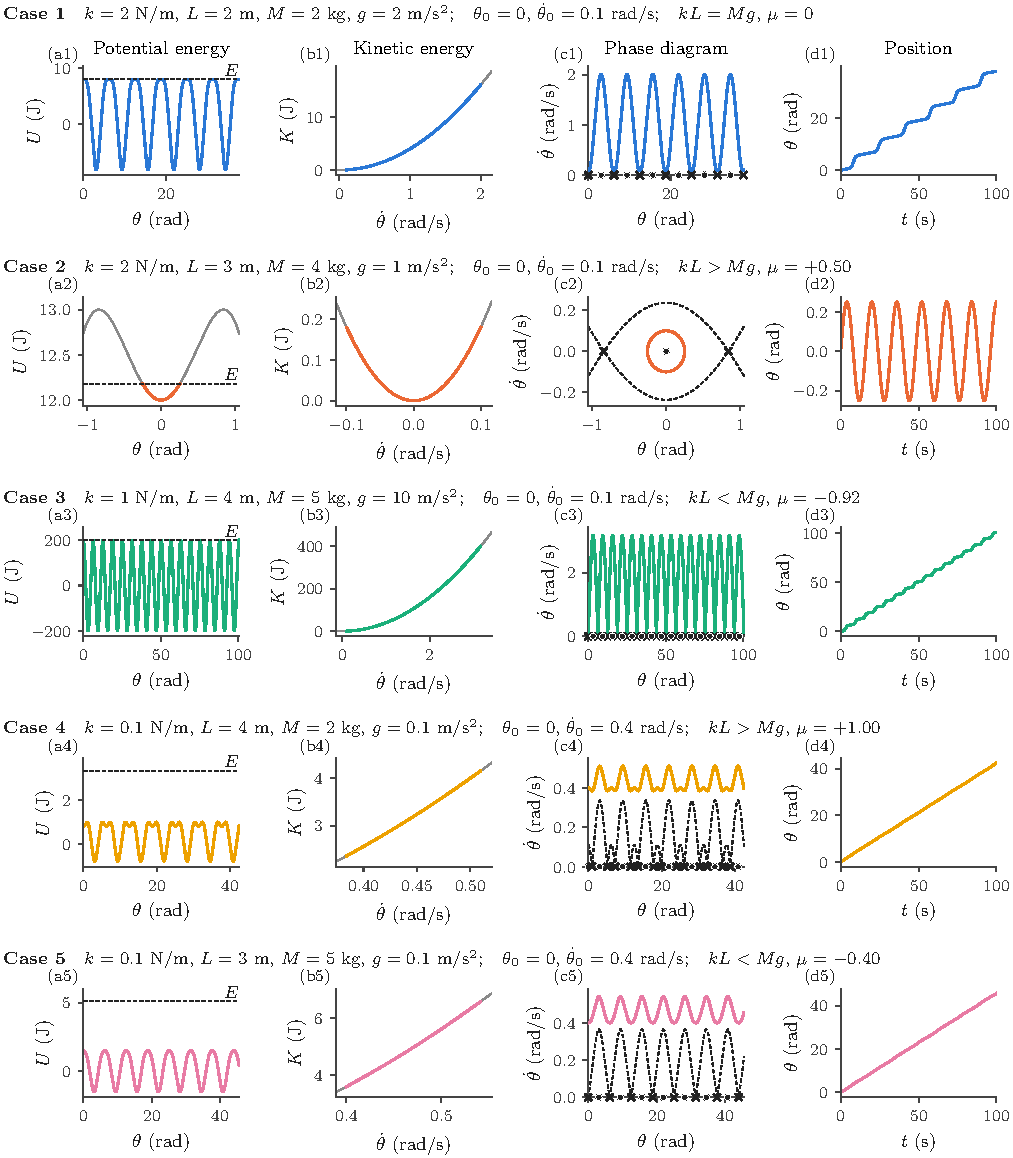
\includegraphics[width=\PIARlayout{0.92\textwidth}{\textwidth}]{figures/fig_cases.pdf}
\caption{Five conservative regimes of Table~\ref{tab:cases}, one case per row. Columns: (a) potential energy along the trajectory as a function of the angle (colored), potential landscape (gray), and total energy $E$ (dashed); (b) kinetic energy as a function of the angular velocity (colored) on the parabola $K=\frac12ML^{2}\dot\theta^{2}$ (gray); (c) phase diagram with the separatrix, Eq.~\eqref{eq:sep_curve} (dashed), centers (dots), and saddles (crosses); (d) position, i.e., the angle, as a function of time over 100~s. For rotations the angle is unwrapped. All curves are drawn from the dense output of DOP853 at 25\,001 instants. Full-size versions of the five rows are given in Figs.~S2--S6 of the supplementary material.}
\label{fig:cases}
\end{figure*}

\subsection{Parameter sets and numerical method}\label{sec:cases_method}

The predictions of Sec.~\ref{sec:model} are illustrated with the five parameter sets listed in Table~\ref{tab:cases}. They cover the three stability classes of the upright position, $kL=Mg$ (case 1), $kL>Mg$ (cases 2 and 4), and $kL<Mg$ (cases 3 and 5), combined with two initial speeds, and their time scales $t_c$ differ by an order of magnitude, from $0.63$ to $6.3$~s, which illustrates the similarity property of Sec.~\ref{sec:units}. Every case starts at the upright position, $\theta_0=0$, with a small angular velocity $\dot\theta_0$ of $0.1$ or $0.4\ \mathrm{rad\,s^{-1}}$. This protocol probes the property that matters most in applications, namely the response of an upright rod to a small kick. The parameters are expressed in SI units, and $g$ is treated as an effective gravitational acceleration: $g=10\ \mathrm{m\,s^{-2}}$ is standard gravity rounded, and the smaller values correspond to a pendulum that moves on a plane inclined by an angle $\alpha$ to the horizontal, for which $g_{\mathrm{eff}}=g\sin\alpha$. Because the dynamics in natural units depends only on $\mu$ (Sec.~\ref{sec:units}), the conclusions apply to every parameter set with the same $\mu$ and the same dimensionless kick $\dot\theta_0t_c$, that is, the same $E/MgL$.

The equation of motion was integrated with the explicit Runge--Kutta method DOP853, of order 8 with error estimators of orders 5 and 3~\cite{HairerNW1993} and built on the coefficients of Prince and Dormand~\cite{PrinceDormand1981}, as implemented in SciPy~\cite{Virtanen2020}, with relative and absolute tolerances of $10^{-12}$ and $10^{-13}$. Each trajectory was then evaluated at 25\,001 equally spaced instants over $100$~s through the continuous extension of order seven that accompanies the method, and all curves of Figs.~\ref{fig:cases} and \ref{fig:portraits} are drawn from this dense output. The mechanical energy, Eq.~\eqref{eq:H}, is conserved to within $8.1\times10^{-11}\,MgL$ in all cases, and the periods measured on the simulated trajectories agree with the quadrature of Eq.~\eqref{eq:period} to a relative accuracy better than $10^{-10}$. As an independent check, the five cases were integrated with the velocity Verlet scheme~\cite{Verlet1967,Swope1982} at a step of $T/2000$ with compensated summation~\cite{Kahan1965}. Because the scheme is symplectic, it conserves a modified Hamiltonian $\tilde H=H+O(h^{2})$, with $h$ the step, up to exponentially small errors over exponentially long times, so that its energy error stays bounded instead of drifting~\cite{BenettinGiorgilli1994,HairerLW2006}; compensated summation keeps the round-off error, which accumulates as a random walk (Brouwer's law~\cite{Brouwer1937}), far below this level. Its energy error remains below $5\times10^{-5}\,MgL$, and its angles agree with the DOP853 trajectories to within $3\times10^{-4}$~rad over the $100$~s.

\subsection{Energy landscapes, phase diagrams, and trajectories}\label{sec:cases_results}

Figure~\ref{fig:cases} presents each case through four complementary views. The first column shows the potential energy along the trajectory, $U(\theta(t))$ as a function of $\theta$, together with the total energy $E$; the part of the landscape that the rod explores, and the margin between $E$ and the peaks of $U$, decide the type of motion. The second column shows the kinetic energy, Eq.~\eqref{eq:K}, as a function of the angular velocity. The curve is always a segment of the parabola $K=\frac12ML^{2}\dot\theta^{2}$, and its extent reveals whether the velocity vanishes at turning points, as in a libration, or never does, as in a rotation. The third column is the phase diagram $(\theta,\dot\theta)$ with the separatrix of Eq.~\eqref{eq:sep_curve}, and the fourth column is the angle as a function of time. For rotations the angle is shown unwrapped, so that one revolution corresponds to an advance of $2\pi$. The cases are discussed from bound to fast motion: the libration (case 2), the two rotations that graze the separatrix (cases 1 and 3), and the two fast rotations (cases 4 and 5).

The upright position is stable in cases 2 and 4, but only in case 2 ($\mu=0.5$) does the rod remain in the upright well. The tilted saddles lie at $\theta^{*}=48.2^{\circ}$, and the energy supplied by the kick, $E=1.015\,MgL$, stays below the top of the barrier, $U(\theta^{*})=1.083\,MgL$. The rod therefore librates inside the upright well [Fig.~\ref{fig:cases}(a2)], with an amplitude of $0.252$~rad ($14.4^{\circ}$), along a closed orbit nested inside the lens-shaped separatrix that joins the two saddles [Fig.~\ref{fig:cases}(c2)]. The motion is nearly harmonic [Fig.~\ref{fig:cases}(d2)], but its period, $16.032$~s, exceeds the linear value $2\pi/\omega_0=15.391$~s by $4.2\%$, i.e., its frequency is lower by $4.0\%$. This lengthening is the signature of the softening cubic term of the normal form, Eq.~\eqref{eq:normal_form}. To first order in the squared amplitude $a^{2}$, the Lindstedt--Poincar\'e method~\cite{Strogatz2015} gives the frequency
\begin{equation}
\omega \simeq \omega_0\left[1-\frac{(3+4\mu)\,a^{2}}{16\,\mu}\right],
\label{eq:lindstedt}
\end{equation}
which predicts, for $a=0.2516$~rad, a frequency shift of $3.96\%$ against the exact $4.00\%$, that is, a period lengthening of $4.1\%$ against the exact $4.2\%$ (Appendix~\ref{app:derivations}).

Case 1 sits exactly at the critical point, $kL=Mg$. The upright position has no linear stiffness, which is the ideal of an isolator, but the quartic maximum $U\simeq MgL(1-\theta^{4}/8)$ makes it unstable, and the kick, which raises the energy only $0.5\%$ above the separatrix, suffices to make the rod rotate. The degenerate maximum produces a striking critical slowing down. Because the potential is flat near the top, the rod creeps across the upright position and then swings rapidly through the hanging one, so that it spends $71\%$ of the time within $45^{\circ}$ of the upright position. The angle advances in a staircase [Fig.~\ref{fig:cases}(d1)], and the orbit hugs the separatrix in the phase diagram [Fig.~\ref{fig:cases}(c1)].

In case 3 ($\mu=-0.92$) the spring is weak, and the upright position is a hyperbolic saddle with growth rate $(\beta|\mu|)^{1/2}=1.52\ \mathrm{s^{-1}}$. The rod departs exponentially from the vertical and rotates with a period of $6.27$~s, completing almost 16 revolutions in 100~s. Its energy exceeds the separatrix energy by only $0.2\%$, so that the orbit again follows the separatrix closely, and the landscape explored in Fig.~\ref{fig:cases}(a3) spans the full range $\pm MgL$. With $\kappa=0.08$, this case is close to the simple pendulum.

In cases 4 and 5 the larger kick, $0.4\ \mathrm{rad\,s^{-1}}$, places the energy far above the separatrix, at $4.2$ and $3.4$ times $MgL$, respectively, and the rod rotates with an angular velocity that never vanishes: the kinetic-energy parabolas of Figs.~\ref{fig:cases}(b4) and \ref{fig:cases}(b5) exclude $\dot\theta=0$, and the angle grows almost linearly in time. The landscapes explain the fine structure of these rotations. For $\mu=1$ (case 4) the potential has a local minimum at the upright position flanked by two maxima at $\theta^{*}=\pm60^{\circ}$, so that the angular velocity dips twice per revolution, whereas for $\mu=-0.4$ (case 5) the only maximum is the upright position and the velocity dips once per revolution [Figs.~\ref{fig:cases}(c4) and \ref{fig:cases}(c5)].

Figure~\ref{fig:portraits} places the five orbits on the phase cylinder, over the occupation densities of long, weakly damped Langevin trajectories at temperature $T_b=0.5\,MgL$ (with Boltzmann's constant set to one), one for each value of $\mu$, integrated with the BAOAB splitting scheme~\cite{LeimkuhlerMatthews2013}. Because the stationary density of Langevin dynamics is the Boltzmann weight $\propto e^{-H/T_b}$, the logarithmic histogram is a map of the energy landscape: it peaks in the hanging well, is depleted near the saddles, and its contours are level curves of $H$, among which the separatrix is the one through the saddles. Cases 1 and 3 run along the separatrix, case 2 is a small closed orbit in the upright well, and cases 4 and 5 are wavy rotations far above it. Taken together, the five cases display the three behaviors that a kicked upright rod can show, namely libration in the upright well, near-separatrix rotation (with critical slowing down at $\mu=0$), and fast rotation, and they confirm that the energy relative to $E_{\mathrm{sep}}$ decides among them.

\begin{figure*}
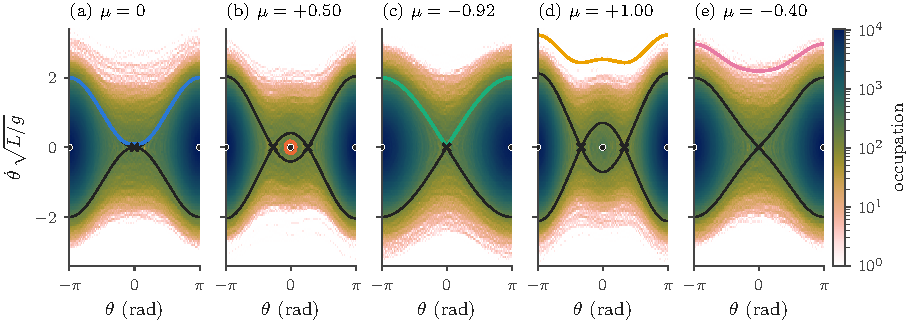
\includegraphics[width=\textwidth]{figures/fig_portraits.pdf}
\caption{Phase portraits of the five cases on the cylinder, in natural units. Panels (a)--(e) correspond to cases 1--5, with the value of $\mu$ in the panel title. Background: occupation histograms of Langevin trajectories at temperature $T_b=0.5\,MgL$, one for each value of $\mu$ (friction $0.02$, time step $0.02$, and $1.2\times10^{7}$ steps; logarithmic color scale, \textit{batlowW}~\cite{Crameri2020}). Black lines: separatrices; colored lines: orbits of the five cases, wrapped to $(-\pi,\pi]$ without spurious jumps; dots and crosses: centers and saddles.}
\label{fig:portraits}
\end{figure*}

\section{Damped--driven dynamics: from the separatrix to a strange attractor}\label{sec:chaos}

\begin{figure*}
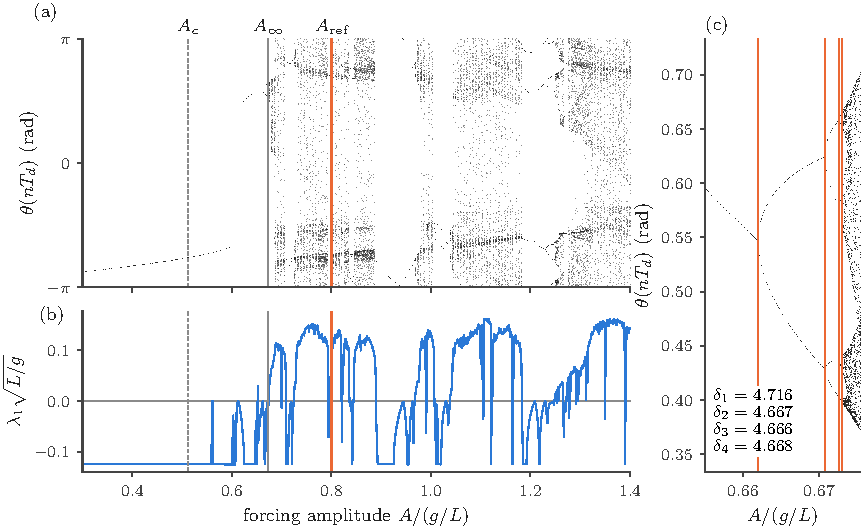
\includegraphics[width=\textwidth]{figures/fig_route.pdf}
\caption{Route to chaos ($\mu=-0.8$, $\gamma=0.25$, $\Omega=2/3$). (a) Stroboscopic bifurcation diagram versus the forcing amplitude; vertical lines mark the Melnikov threshold $A_c$ of Sec.~\ref{sec:melnikov} (dashed), the accumulation point $A_\infty$ of the period-doubling cascade, and the reference chaotic state $A_{\mathrm{ref}}=0.8$. (b) Largest Lyapunov exponent. (c) Magnification of the cascade; vertical lines mark the first four thresholds obtained by Floquet continuation, and the ratios of Eq.~\eqref{eq:feigenbaum} are listed.}
\label{fig:route}
\end{figure*}

\subsection{Forced model and symmetry}\label{sec:forced_model}

Real isolators dissipate energy and are driven by their environment. Both effects are introduced by adding viscous damping and a harmonic torque to Eq.~\eqref{eq:eom},
\begin{equation}
\ddot\theta + \gamma\dot\theta + \lambda\sin\theta\cos\theta - \beta\sin\theta = A\cos\Omega t ,
\label{eq:forced}
\end{equation}
where $\gamma$ is the damping rate, $A$ is the torque amplitude per unit moment of inertia, and $\Omega$ is the angular frequency of the drive. Because the right-hand side depends explicitly on time, the phase space is extended to $S^{1}\times\mathbb R\times S^{1}$ by the forcing phase $\Omega t$, and the divergence of the flow is the constant $-\gamma$. Phase-space volumes therefore contract exponentially, and the long-time dynamics settles on an attractor. The reflection symmetry of Sec.~\ref{sec:separatrix} survives in a spatiotemporal form: Eq.~\eqref{eq:forced} is invariant under
\begin{equation}
(\theta,t)\to(-\theta,\,t+\pi/\Omega),
\label{eq:st_symmetry}
\end{equation}
that is, under a reflection combined with a shift by half a forcing period. This symmetry constrains the sequence of bifurcations~\cite{SwiftWiesenfeld1984} and, as shown in Sec.~\ref{sec:identifiability}, determines the role of the forcing phase in the reconstruction. A harmonic acceleration $\ddot x_g$ of the base, which is the excitation relevant to seismic isolation, would instead enter as $-(\ddot x_g/L)\cos\theta$; it has the same symmetry but acts multiplicatively, and it is left for future work.

The analysis uses $\mu=-0.8$ ($\kappa=0.2$), $\gamma=0.25$, and $\Omega=2/3$ in natural units, with the amplitude $A$, in units of $g/L$, as the control parameter. For $\mu<0$ the upright saddle carries a homoclinic loop around the cylinder, the natural seed of chaos analyzed in Sec.~\ref{sec:melnikov}, and the model connects continuously with the damped--driven pendulum ($\mu\to-1$), whose route to chaos is well documented; the chosen values define a weakly spring-loaded version of the pendulum studied by Baker and Gollub~\cite{BakerGollub1996}, with the same drive frequency. The isolator regime, $\mu\gtrsim0$, is better served by the base-excited model and is not treated here. Trajectories were integrated with a fixed-step fourth-order Runge--Kutta (RK4) scheme with 128 steps per forcing period $T_d=2\pi/\Omega$ (256 for the Floquet continuation and 96 for the Lyapunov chart of Sec.~\ref{sec:melnikov}), together with the variational equations whenever the tangent dynamics was required. Lyapunov exponents are denoted $\lambda_i$ and are distinct from $\lambda=k/M$.

\subsection{Route to chaos}\label{sec:route}

The stroboscopic Poincar\'e map, $P:\mathbf z(t_0)\mapsto\mathbf z(t_0+T_d)$ with $\mathbf z=(\theta,\dot\theta)$, reduces the flow to a two-dimensional map that contracts areas uniformly, $\det DP=e^{-2\pi\gamma/\Omega}$, a property verified to within $10^{-8}$ for the monodromy matrix computed with 256 steps per forcing period. Its bifurcation diagram [Fig.~\ref{fig:route}(a)], computed for 1101 amplitudes $A\in[0.30,1.40]$ after a transient of 300 forcing periods, shows the familiar alternation of periodic windows and chaotic bands. For $1.8\%$ of the amplitudes the period of the attractor differs between upward and downward sweeps of $A$, a signature of coexisting attractors.

A period doubling occurs when a Floquet multiplier of a periodic orbit crosses $-1$. To locate these points, periodic orbits were computed by Newton iteration on $P^{n}(\mathbf z)=\mathbf z$, with the monodromy matrix taken from the variational equations, and continued in $A$~\cite{ParkerChua1989,Kuznetsov2004}. The cascade starts from one of two asymmetric period-1 orbits that are mirror images of each other under Eq.~\eqref{eq:st_symmetry}, since a symmetric orbit must break the symmetry before it can double its period~\cite{SwiftWiesenfeld1984}; the mirror orbit coexists as a separate attractor. Six successive doublings $A_1<\dots<A_6$ were tracked in this way (Table~\ref{tab:chaos}). The ratios of successive intervals,
\begin{equation}
\delta_n = \frac{A_{n+1}-A_{n}}{A_{n+2}-A_{n+1}},
\label{eq:feigenbaum}
\end{equation}
take the values $4.716$, $4.667$, $4.666$, and $4.668$ [Fig.~\ref{fig:route}(c)], in agreement with Feigenbaum's universal constant $\delta=4.6692$~\cite{Feigenbaum1978}. Geometric extrapolation with this universal ratio places the accumulation point at $A_\infty=0.673239$, beyond which chaotic bands appear.

The largest Lyapunov exponent measures the mean exponential rate at which nearby trajectories separate,
\begin{equation}
\lambda_1 = \lim_{t\to\infty}\frac1t\ln\frac{\|\delta\mathbf z(t)\|}{\|\delta\mathbf z(0)\|},
\label{eq:lyapunov}
\end{equation}
where $\delta\mathbf z$ is an infinitesimal perturbation of the state evolved by the variational equations. It was computed with the algorithm of Benettin et al., with QR reorthonormalization~\cite{Benettin1980,Benettin1980b}, over 1500 forcing periods at every amplitude [Fig.~\ref{fig:route}(b)], and it exceeds $10^{-3}$ for $45\%$ of the scanned amplitudes. Because the extended flow has a neutral direction along time ($\lambda_2=0$) and the constant divergence $-\gamma$, the other two exponents obey the sum rule $\lambda_1+\lambda_3=-\gamma$, which holds to within $3.3\times10^{-7}$ over the whole scan; because the trace of the variational matrix equals $-\gamma$ for every state, this checks the volume contraction of the integrated tangent map rather than the value of $\lambda_1$ itself.

\subsection{Splitting of the separatrix}\label{sec:melnikov}

The bifurcation diagram shows where chaos appears; the geometry of the conservative system explains why. For $\mu<0$ the upright saddle is connected to itself by a homoclinic orbit $\theta_h(t)$, the separatrix of Eq.~\eqref{eq:Esep_neg}, which winds once around the cylinder; its time origin is fixed at the bottom of the loop. In the conservative system the stable and unstable manifolds of the saddle coincide along this orbit; damping and forcing split them, and whether the split manifolds intersect decides whether chaos is possible. To first order in $\gamma$ and $A$, the signed distance between the manifolds on the section $t=t_0$ is proportional to the Melnikov function~\cite{Melnikov1963,GuckenheimerHolmes1983}
\begin{equation}
\mathcal M(t_0) = -\gamma I_0 + A\,I_1(\Omega)\cos\Omega t_0,
\label{eq:melnikov}
\end{equation}
with
\begin{equation}
I_0 = \int_{-\infty}^{\infty}\dot\theta_h^{2}\,\mathrm dt,\qquad
I_1(\Omega) = \int_{-\infty}^{\infty}\dot\theta_h\cos\Omega t\,\mathrm dt .
\label{eq:melnikov_integrals}
\end{equation}
The first term of Eq.~\eqref{eq:melnikov} is the energy dissipated by friction along the homoclinic loop, and the second is the work done by the drive along the loop. When the work can exceed the dissipation, that is, for
\begin{equation}
\frac{A}{\gamma} > \left(\frac{A}{\gamma}\right)_{\!c} = \frac{I_0}{|I_1(\Omega)|},
\label{eq:melnikov_threshold}
\end{equation}
the function $\mathcal M$ has simple zeros, the manifolds intersect transversally, and the Smale--Birkhoff theorem guarantees a horseshoe, hence at least transient chaos~\cite{GuckenheimerHolmes1983}. For the PIAR both integrals have closed forms (Appendix~\ref{app:derivations}). For $\kappa=0.2$ and $\Omega=2/3$ they give $I_0=7.725$, $I_1=3.770$, and $(A/\gamma)_c=2.049$, i.e., $A_c=0.512$ for $\gamma=0.25$, and in the pendulum limit $\kappa\to0$ the classic threshold $(A/\gamma)_c=(4/\pi)\cosh(\pi\Omega/2)$ is recovered. The criterion is first order in the perturbation and neither necessary nor sufficient for a chaotic attractor, but it is borne out by a chart of the largest Lyapunov exponent in the $(A,\Omega)$ plane [Fig.~\ref{fig:attractor}(c)]: none of the chaotic cells lies below the Melnikov curve, whereas $26.7\%$ of the cells above it are chaotic. In this precise sense, the strange attractor of the damped--driven PIAR grows out of the separatrix of the conservative one.

\subsection{The reference strange attractor}\label{sec:attractor}

The chaotic state at $A=0.8$ is the attractor that the reconstruction of Secs.~\ref{sec:fprm} and \ref{sec:results} must recover. Its orbit wanders around the ghost of the conservative separatrix, alternating between rotations and librations in an unpredictable sequence [Fig.~\ref{fig:attractor}(a), drawn through a cubic Hermite interpolant between integration steps; Sec.~\ref{sec:lab}], and its invariant measure on the stroboscopic section displays the folded, fractal structure of a strange attractor [Fig.~\ref{fig:attractor}(b)]. Ten independent runs of 5000 forcing periods give $\lambda_1=0.0956\pm0.0008$ (standard error) and $\lambda_3=-0.3456$, which sum to $-0.2500$. The Lyapunov time, $1/\lambda_1=10.5$ natural time units, is about one forcing period, and an error of the size of the measurement noise used below, $0.01$, grows to the size of the signal in about $\ln100\approx4.6$ Lyapunov times, i.e., five forcing periods. Long gaps in a record therefore cannot be bridged by extrapolating the past of the same signal: the missing information must come from a concurrent, complete channel, which is precisely the premise of the FPRM.

The exponents also fix the dimension of the attractor. The Kaplan--Yorke dimension~\cite{KaplanYorke1979},
\begin{equation}
D_{\mathrm{KY}} = 2 + \frac{\lambda_1}{|\lambda_3|} = 2.277 ,
\label{eq:dky}
\end{equation}
is the dimension of the flow ($1.277$ on the Poincar\'e section), and the correlation dimension of the section, computed with the Grassberger--Procaccia algorithm~\cite{Grassberger1983} and fitted over $10^{-4}\le r\le2\times10^{-3}$, is $D_2=1.13$, consistent with $D_2\le D_{\mathrm{KY}}-1$ on the section. These values set the embedding dimension that suffices according to the reconstruction theorems of Sec.~\ref{sec:takens}. A delay embedding of dimension $d_E>2D_0$, with $D_0$ the box-counting dimension of the attractor, is generically one-to-one~\cite{Sauer1991}. With $D_0\simeq D_{\mathrm{KY}}$, the dimension $d_E=5$ exceeds this bound only by a small margin; for the spring force, the fraction of false nearest neighbors indeed falls to $0.9\%$ at $d_E=5$ (Sec.~\ref{sec:tasks}).

The attractor is, finally, symmetric. The stroboscopic section at phase zero agrees with the mirror image of the section taken half a forcing period later: for three records of $2\times10^{5}$ forcing periods, the total-variation distance between their histograms is $0.013$--$0.018$, comparable to the distance of $0.013$--$0.015$ between the sections of two independent records of the same length, which measures the sampling noise, and the time averages of $\sin\theta$ and $\dot\theta$ vanish to within $2\times10^{-3}$ (Table~S9 of the supplementary material). Every state of the attractor is therefore accompanied by its image under Eq.~\eqref{eq:st_symmetry}, with the opposite angle and angular velocity and a forcing phase shifted by $\pi$.

Three properties of the attractor thus define the reconstruction problem addressed next. Its Lyapunov time limits how long a gap can be bridged from the incomplete record alone; its dimension fixes how much history of the complete channel must be retained; and its symmetry decides which channels can stand in for which, since a channel that is invariant under the reflection, such as the collar height, cannot, on its own, distinguish a state from its mirror image unless the phase of the forcing is also known. Section~\ref{sec:fprm} turns these three properties into the design of the reconstruction.

\begin{table}
\caption{Characterization of the damped--driven PIAR ($\mu=-0.8$, $\gamma=0.25$, $\Omega=2/3$; natural units). The Lyapunov exponents, the Lyapunov time, and the dimensions refer to the reference state $A=0.8$; $A_\infty$ is extrapolated with Feigenbaum's constant.}
\label{tab:chaos}
\begin{ruledtabular}
\begin{tabular}{@{}lr@{}}
Quantity & Value\\
\hline
Doublings $A_1$, $A_2$ & 0.66200641, 0.67085169\\
Doublings $A_3$, $A_4$ & 0.67272715, 0.67312902\\
Doublings $A_5$, $A_6$ & 0.67321514, 0.67323359\\
Ratios $\delta_1,\dots,\delta_4$ & 4.716, 4.667, 4.666, 4.668\\
Accumulation point $A_\infty$ & 0.673239\\
Melnikov integrals $I_0$, $I_1$ & 7.725, 3.770\\
Melnikov threshold $(A/\gamma)_c$, $A_c$ & 2.049, 0.512\\
Exponents $\lambda_1$, $\lambda_3$ & $0.0956(8)$, $-0.3456$\\
Lyapunov time $1/\lambda_1$ & 10.5 ($1.1\,T_d$)\\
$D_{\mathrm{KY}}$ (flow, section) & 2.277, 1.277\\
$D_2$ (section) & 1.13\\
\end{tabular}
\end{ruledtabular}
\end{table}

\begin{figure*}
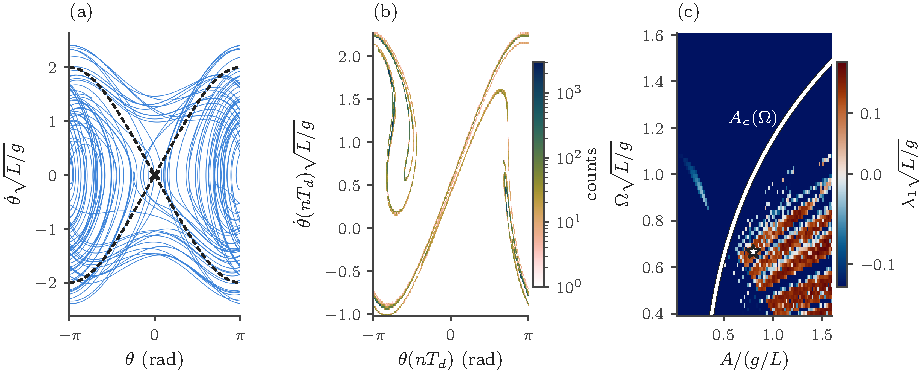
\includegraphics[width=\textwidth]{figures/fig_attractor.pdf}
\caption{The reference strange attractor ($A=0.8$). (a) Forty forcing periods of the chaotic orbit on the phase cylinder, drawn through the cubic Hermite interpolant, with the separatrix of the conservative system (dashed) and the upright saddle (cross). (b) Invariant measure on the stroboscopic section: logarithmic histogram of $2\times10^{5}$ points. (c) Largest Lyapunov exponent in the $(A,\Omega)$ plane (diverging colormap \textit{vik}~\cite{Crameri2020}, centered at zero; $90\times70$ cells with 150 transient and 400 recorded periods) and Melnikov threshold $A_c(\Omega)=\gamma I_0/|I_1(\Omega)|$ (white); the star marks the reference state.}
\label{fig:attractor}
\end{figure*}

\section{The full--partial reconstruction mapping}\label{sec:fprm}

\begin{figure*}
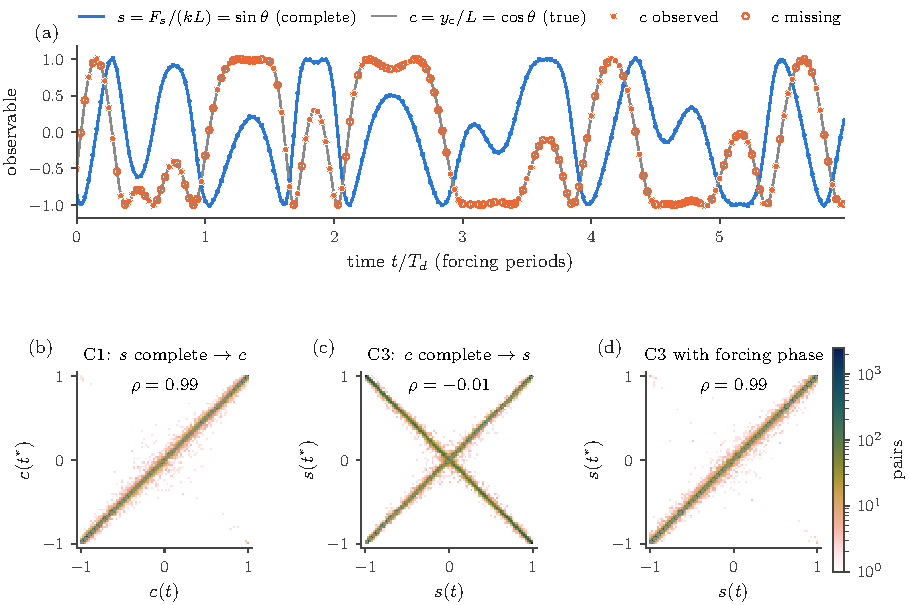
\includegraphics[width=\textwidth]{figures/fig_fprm_scheme.pdf}
\caption{The reconstruction problem on the chaotic attractor ($\mu=-0.8$, $\gamma=0.25$, $A=0.8$, $\Omega=2/3$). (a) Measurable observables over six forcing periods: the complete spring-force channel $s$ and the collar-height channel $c$ with $60\%$ of its entries missing (open circles); lines are the continuous trajectories and dots the noisy samples. (b)--(d) Model-free identifiability test (task labels as in Sec.~\ref{sec:tasks}): target value at time $t$ versus its value at the time $t^{\ast}$ of the nearest neighbor of the delay vector of the complete channel (logarithmic histograms of $4\times10^{4}$ pairs, with temporal neighbors closer than one forcing period excluded). (b) $s$ complete, $c$ target: identifiable. (c) $c$ complete, $s$ target: the reflection symmetry creates a mirror branch. (d) As (c), with the forcing phase appended to the delay vector: identifiability is restored.}
\label{fig:fprm_scheme}
\end{figure*}

The attractor of Sec.~\ref{sec:attractor} is never observed as such: sensors record scalar functions of the state, such as the spring force or the height of the collar, and some of these records are incomplete. The reconstruction method is therefore developed in the order dictated by the three properties identified there. The delay reconstruction, which replaces the unobserved state by the history of one complete channel, is introduced first (Sec.~\ref{sec:takens}), followed by the FPRM, which maps this history onto the missing channel (Sec.~\ref{sec:fprm_framework}). The identifiability conditions imposed by the symmetry are then derived and tested on data (Sec.~\ref{sec:identifiability}), and the generative engine and the physical constraints proposed here are presented (Secs.~\ref{sec:flow} and \ref{sec:physics_reg}), before the reconstruction tasks and the metrics are defined (Sec.~\ref{sec:tasks}). In brief, task C1 reconstructs the collar height and the angular velocity from the complete spring force on the chaotic attractor; task C2 reconstructs the spring force from the complete collar height of an undriven, stochastic PIAR; task C3 does so on the chaotic attractor, with and without the forcing phase; and task C0 is a trivial control.

\subsection{Delay reconstruction}\label{sec:takens}

The state $\mathbf z(t)$ of a dynamical system is assumed to settle on an attractor $\mathcal A$ and to be observed through a scalar measurement $x(t)=\mathcal O(\mathbf z(t))$, such as the spring force. The delay vector
\begin{equation}
\mathbf x(t) = \bigl[x(t),\,x(t-\tau),\,\dots,\,x(t-(d_E-1)\tau)\bigr]\in\mathbb R^{d_E},
\label{eq:delay}
\end{equation}
built from $d_E$ samples separated by a delay $\tau$, defines the delay map $\Phi_x:\mathbf z(t)\mapsto\mathbf x(t)$. Takens' theorem~\cite{Takens1981}, in the form extended to fractal attractors by Sauer, Yorke, and Casdagli~\cite{Sauer1991}, states that the delay map is one-to-one on the attractor for a generic measurement function $\mathcal O$ whenever $d_E>2D_0$, where $D_0$ is the box-counting dimension of $\mathcal A$; the extension to periodically forced systems, in which the phase of the drive is part of the state, is due to Stark~\cite{Stark1999}. The reconstructed set $\mathcal A_x=\Phi_x(\mathcal A)$ is then a faithful copy of the original attractor: distinct states have distinct delay vectors, and the history of a single variable encodes the whole state~\cite{Packard1980,Abarbanel1993}. In practice the delay is chosen at the first minimum of the average mutual information between $x(t)$ and $x(t-\tau)$~\cite{FraserSwinney1986}, and the dimension by the method of false nearest neighbors~\cite{Kennel1992}, which increases $d_E$ until points that are neighbors in $\mathbb R^{d_E}$ remain neighbors in $\mathbb R^{d_E+1}$~\cite{KantzSchreiber2004}.

\subsection{The mapping between full and partial reconstructions}\label{sec:fprm_framework}

The FPRM~\cite{Wu2026FPRM} considers two observables of the same system: a completely observed channel $x$ and a partially observed channel $y$ with missing entries. Their delay reconstructions, $\mathcal A_F=\Phi_x(\mathcal A)$ (full) and $\mathcal A_P=\Phi_y(\mathcal A)$ (partial), are both one-to-one images of the attractor, so that the map
\begin{equation}
\Psi = \Phi_y\circ\Phi_x^{-1}:\ \mathcal A_F\to\mathcal A_P
\label{eq:fprm_map}
\end{equation}
is well defined and continuous. In particular, the current value of the incomplete channel is a function of the delay vector of the complete one,
\begin{equation}
y(t) = \psi\bigl(\mathbf x(t)\bigr),
\label{eq:fprm_function}
\end{equation}
where $\psi$ is the first component of $\Psi$. The function $\psi$ can be learned from the pairs $(\mathbf x(t),y(t))$ at the times at which $y$ is observed and evaluated at the times at which it is missing. This is the essence of the method, which is closely related to the cross mapping between reconstructed manifolds used to detect causal coupling~\cite{Sugihara2012}.

In the original formulation, $\psi$ is learned by Gaussian-process regression~\cite{Rasmussen2006}. A zero-mean Gaussian-process prior with covariance function $\mathcal K(\mathbf x,\mathbf x')$ is placed on $\psi$, and, given $N$ training inputs with noisy outputs $\mathbf y=(y_1,\dots,y_N)^{\top}$, the prediction at a new input $\mathbf x_*$ is the Gaussian distribution with mean and variance
\begin{equation}
\begin{aligned}
\bar\psi(\mathbf x_*) &= \mathbf k_*^{\top}(\mathbf K+\sigma_n^{2}I)^{-1}\mathbf y,\\
\sigma_*^{2}(\mathbf x_*) &= \mathcal K(\mathbf x_*,\mathbf x_*) - \mathbf k_*^{\top}(\mathbf K+\sigma_n^{2}I)^{-1}\mathbf k_* .
\end{aligned}
\label{eq:gpr}
\end{equation}
Here $\mathbf K$, with entries $\mathcal K(\mathbf x_i,\mathbf x_j)$, is the covariance matrix of the training inputs, $\mathbf k_*$ is the vector of covariances between $\mathbf x_*$ and the training inputs, $\sigma_n^{2}$ is the noise variance, and $I$ is the identity matrix; the mean $\bar\psi$ is the imputed value, and $\sigma_*$ its uncertainty. With a squared-exponential covariance and one length scale per delay coordinate, the hyperparameters are fitted by maximizing the marginal likelihood of the training data. In the implementation used here, the fitted noise variance is added to $\sigma_*^{2}$, so that the predictive distribution refers to a new noisy observation; when the marginal likelihood attributes most of the variance to noise, the prediction becomes broad. The approach is elegant and data-efficient, and it recovers complex dynamics at large missing fractions~\cite{Wu2026FPRM}. Its predictive distribution, however, is a single Gaussian, and this restriction becomes decisive whenever Eq.~\eqref{eq:fprm_function} fails.

\subsection{Identifiability and symmetry}\label{sec:identifiability}

Equation~\eqref{eq:fprm_function} rests on the assumption that the delay map of the complete channel is one-to-one, and symmetries can violate it~\cite{LetellierAguirre2002,Letellier2005}. If a transformation $R$ of the state space commutes with the flow, maps the attractor onto itself, and leaves the complete channel invariant, $x\circ R=x$, but changes the incomplete one, $y\circ R\ne y$, then a state and its image under $R$ produce the same delay vector while carrying different values of $y$. The missing value is then not a function of $\mathbf x(t)$, and its conditional distribution $p(y\mid\mathbf x)$ has one branch for each member of the symmetry orbit. The PIAR realizes this situation in its simplest form. By Eq.~\eqref{eq:reflection}, the collar height $c$ is invariant under the reflection $(\theta,\dot\theta)\to(-\theta,-\dot\theta)$ while the spring force $s$ changes sign, so that in the autonomous system no record of $c$ can determine the sign of $s$, and the conditional distribution of $s$ is bimodal, with branches $s=\pm(1-c^{2})^{1/2}$. The converse task is well posed: $s$ is invariant only under $\theta\to\pi-\theta$, which exchanges the upper and lower half-planes and is not a symmetry of the dynamics, because gravity distinguishes up from down. In the driven system the reflection is a symmetry only when combined with a half-period time shift, Eq.~\eqref{eq:st_symmetry}. Two states related by this symmetry experience forcing phases that differ by $\pi$, and appending the phase $(\cos\Omega t,\sin\Omega t)$ to the delay vector therefore restores the one-to-one property. Stark's forced embedding theorem~\cite{Stark1999} does not require the phase to be observed, but it holds only for generic observables, and $c$ is not generic because it is invariant under Eq.~\eqref{eq:st_symmetry}.

These statements can be tested directly on data, before any model is trained, with the simplest possible estimate of $\psi$: the value of the incomplete channel at the nearest neighbor of $\mathbf x(t)$ on $\mathcal A_F$. Tests of this kind, which ask whether neighbors in one reconstruction remain neighbors in another, have long been used to detect continuity and generalized synchronization between time series~\cite{Pecora1995,Rulkov1995}. Figure~\ref{fig:fprm_scheme} shows the result for the chaotic attractor of Sec.~\ref{sec:attractor}, computed from the complete channel, with measurement noise of standard deviation $0.01$, the noise-free target channel, and the embeddings selected in Sec.~\ref{sec:tasks}; neighbors closer in time than one forcing period were excluded, as recommended by Theiler~\cite{Theiler1986}. When the spring force is complete and the collar height is the target, the neighbor predicts the target almost perfectly (correlation $\rho=0.99$), and the scatter collapses onto the diagonal [Fig.~\ref{fig:fprm_scheme}(b)]. When the roles are exchanged, the scatter forms an X: the neighbor carries either the correct value or its mirror image with equal probability, and the correlation vanishes [$\rho=-0.01$; Fig.~\ref{fig:fprm_scheme}(c)]. Appending the forcing phase removes the mirror branch and restores $\rho=0.99$ [Fig.~\ref{fig:fprm_scheme}(d)]. The identifiability of every reconstruction task is thus established in advance, from the symmetry of the model and from a model-free test.

\subsection{Generative engine: A conditional normalizing flow}\label{sec:flow}

To represent ambiguous targets, the FPRM is recast here as conditional density estimation: instead of a function $\psi$, a conditional distribution $q_\phi(y\mid\mathbf h)$ with parameters $\phi$ is learned, and imputations are drawn from it. For the sample recorded at time $t_n$, the conditioning vector
\begin{equation}
\begin{split}
\mathbf h_n = \bigl[\,&x_{n-m\tau},\dots,x_{n+m\tau};\ \tilde y_{n\pm1},\dots,\tilde y_{n\pm n_b};\\
&\mathfrak m_{n\pm1},\dots,\mathfrak m_{n\pm n_b};\ \cos\Omega t_n,\ \sin\Omega t_n\,\bigr]
\end{split}
\label{eq:context}
\end{equation}
collects all the information available at that sample, with subscripts counting samples and the delay $\tau$ expressed in samples. Its first block is a symmetric window of the complete channel with $2m+1$ samples spaced by $\tau$, where $m=\lceil(d_E-1)/2\rceil$; it is a delay vector of dimension $2m+1\ge d_E$ centered at $t_n$, which is admissible because the reconstruction is performed offline. The second and third blocks contain the neighbors of the incomplete channel, $n_b=3$ samples on each side, set to zero where missing ($\tilde y$), together with the corresponding availability mask $\mathfrak m$; they allow the model to exploit continuity when some neighbors are observed. The last block, the forcing phase, is included in task C1 and in the phase variant of task C3 (Sec.~\ref{sec:tasks}).

The conditional density is represented by a normalizing flow~\cite{Papamakarios2021}, which writes the target, of dimension $d_y$ (one or two), as an invertible transformation of a standard normal variable, $y=\mathcal G_\phi(\mathbf u;\mathbf h)$ with $\mathbf u\sim\mathcal N(\mathbf 0,I)$ in $\mathbb R^{d_y}$. The change-of-variables formula then gives the exact density,
\begin{equation}
\ln q_\phi(y\mid\mathbf h) = \ln\mathcal N\bigl(\mathcal G_\phi^{-1}(y;\mathbf h)\bigr) + \ln\left|\det\frac{\partial \mathcal G_\phi^{-1}(y;\mathbf h)}{\partial y}\right| ,
\label{eq:flow}
\end{equation}
in which the first term is the base density evaluated at the preimage of $y$ and the second accounts for the local stretching of volumes by the transformation. A neural spline flow (NSF)~\cite{Durkan2019} is used, in which $\mathcal G_\phi$ is a composition of three autoregressive transforms, each a monotonic rational-quadratic spline with eight bins whose knots are produced by a neural network that receives the conditioning vector; the implementation relies on \texttt{zuko}~\cite{zuko} and PyTorch~\cite{Paszke2019}. The parameters are trained by maximizing the log-likelihood of Eq.~\eqref{eq:flow} over the observed pairs $(\mathbf h_n,y_n)$, missing entries are imputed by sampling, and the posterior median is used whenever a point estimate is required.

A flow was chosen as the main engine for three reasons, two of which are quantified against the diffusion model in Sec.~\ref{sec:res_engine}. It provides the exact likelihood of Eq.~\eqref{eq:flow}, a proper criterion for selecting the model on held-out data, whereas the conditional variational autoencoder and the diffusion model introduced below are validated through a bound or a surrogate of their likelihood; it generates each sample with a small, fixed number of network evaluations instead of an iterative denoising chain; and its samples are differentiable functions of the parameters, obtained in the same pass, which makes the physical constraints described next affordable. One limitation should be anticipated: because a flow is a diffeomorphism of $\mathbb R^{d_y}$, a flow with a unimodal Gaussian base must connect separated modes by thin bridges of probability~\cite{Cornish2020}.

For comparison, two other conditional generative models receive the same conditioning vector: a conditional variational autoencoder (cVAE)~\cite{Kingma2014,Sohn2015}, which maximizes a lower bound on the likelihood through a latent Gaussian variable, and a conditional denoising diffusion probabilistic model (DDPM)~\cite{Ho2020,NicholDhariwal2021}, which learns to invert a gradual noising process and underlies the conditional score-based diffusion imputer (CSDI)~\cite{Tashiro2021}.

\subsection{Physics-informed regularization}\label{sec:physics_reg}

The equation of motion, Eq.~\eqref{eq:forced}, is known in form, and the question is whether imposing it on the imputations improves them. The known mechanics enters, as in physics-informed neural networks~\cite{Raissi2019}, through residuals evaluated on reparameterized samples $\hat y\sim q_\phi(\cdot\mid\mathbf h_n)$~\cite{Kingma2014}, so that gradients propagate through the flow. For the task in which $s$ is complete and the collar height $c$ and the angular velocity $v=\dot\theta$ are imputed (task C1 of Sec.~\ref{sec:tasks}), three residuals vanish for the true values:
\begin{align}
r_{\mathrm{hol}} &= \hat c^{2}+s^{2}-1, \label{eq:res_hol}\\
r_{\mathrm{kin}} &= \hat c\,\hat v - \dot s, \label{eq:res_kin}\\
r_{\mathrm{EOM}} &= \ddot s + s\,\hat v^{2} - \hat c\,\bigl[\beta s - \lambda s\hat c - \gamma\hat v + f(t)\bigr], \label{eq:res_eom}
\end{align}
where $\hat c$ and $\hat v$ are the imputed values and $f(t)=A\cos\Omega t$ is the drive. The holonomic residual, Eq.~\eqref{eq:res_hol}, states that $(s,c)$ lies on the unit circle. The kinematic residual, Eq.~\eqref{eq:res_kin}, follows from differentiating $s=\sin\theta$, which gives $\dot s=\cos\theta\,\dot\theta$. The dynamical residual, Eq.~\eqref{eq:res_eom}, is the equation of motion multiplied by $\cos\theta$ and rewritten with the identity $\ddot s=\cos\theta\,\ddot\theta-\sin\theta\,\dot\theta^{2}$, so that it contains only the observed channel, its derivatives, and the imputed quantities. For the driven task in which $c$ is complete and $s$ is imputed (C3), the holonomic residual $\hat s^{2}+c^{2}-1$ is complemented by the equation of motion expressed through $c$, its derivatives, and $\hat s$, multiplied by $\sin^{3}\theta$ to remove the singular factor $1/\sin\theta$ of $\dot\theta=-\dot c/\sin\theta$ (Appendix~\ref{app:derivations}),
\begin{equation}
r_{\mathrm{EOM}} = -\hat s^{2}\ddot c - c\,\dot c^{2} - \gamma\dot c\,\hat s^{2} + \lambda\hat s^{4}c - \beta\hat s^{4} - f(t)\,\hat s^{3}.
\label{eq:res_c3}
\end{equation}
The same residual, which contains the known drive $f(t)$ at the true sample times, is used in both variants of C3, so that in the variant without the phase the physics term carries timing information that the conditioning vector lacks. In the stochastic task C2 only the holonomic residual is imposed, because the random force of the Langevin dynamics has no deterministic counterpart in the equation of motion.

Derivatives of the complete channel are estimated with Savitzky--Golay filters~\cite{SavitzkyGolay1964} (window of 7 samples, degree 4). Residuals computed from noisy derivatives cannot vanish exactly, and forcing them to zero oversharpens the conditional density. Each residual $r_j$, with $j\in\{\mathrm{hol},\mathrm{kin},\mathrm{EOM}\}$, is therefore scaled by its root-mean-square value $\sigma_j$ at the observed data, and only the part with $|r_j|>2\sigma_j$ is penalized, which yields the training objective
\begin{equation}
\begin{split}
J(\phi) = &-\bigl\langle\ln q_\phi(y_n\mid\mathbf h_n)\bigr\rangle_{\mathrm{obs}}\\
&+ w\,\Bigl\langle\sum_j \mathrm{ReLU}\bigl(r_j^{2}/\sigma_j^{2}-4\bigr)\Bigr\rangle_{\mathrm{coll},\,\hat y}.
\end{split}
\label{eq:loss}
\end{equation}
The first average runs over the observed pairs and is the negative log-likelihood; the second runs over collocation times and samples, $\mathrm{ReLU}(\cdot)=\max(\cdot,0)$, and the weight $w=1$ is ramped in linearly between $10\%$ and $20\%$ of the training budget. The collocation times are drawn from all time indices, including those whose target is missing: because the residuals depend only on the complete channel and on the samples, this adds information precisely where imputation is required, without using any held-out value. One property of these residuals is decisive for what follows. In tasks C2 and C3 the holonomic residual is invariant under $\hat s\to-\hat s$, and in C3 only the forcing term of Eq.~\eqref{eq:res_c3} is odd in $\hat s$, so that the physics can discriminate between mirror branches only through the drive. In task C1 the relevant mirror is $(\hat c,\hat v)\to(-\hat c,-\hat v)$, which leaves $s$ and $\dot s$ unchanged; under it, only the gravitational and forcing terms of Eq.~\eqref{eq:res_eom} change sign, so that the physics can locate the rod in the upper or lower half-plane.

\subsection{Reconstruction tasks, data, and metrics}\label{sec:tasks}

The tasks follow from the identifiability analysis of Sec.~\ref{sec:identifiability}. Reconstructing $\dot\theta$ from a complete record of $\theta$ is solved by numerical differentiation and is retained only as a control (C0). Three informative tasks use the measurable observables $s$ and $c$. In task C1 the spring force is complete, and the collar height and the angular velocity are missing at the same instants, as happens when both are derived from a single angle-encoder record; this target is identifiable, and the angular velocity cannot be obtained by differentiating the observed channel alone. In task C2 the collar height of an autonomous, stochastic PIAR is complete and the spring force is missing, so that the target is not identifiable by symmetry. Task C3 is the driven analogue of C2, with and without the forcing phase in the conditioning vector.

Tasks C1 and C3 use the reference attractor of Sec.~\ref{sec:attractor}, sampled 32 times per forcing period ($\Delta t=0.295$) for $4\times10^{4}$ samples after a transient of 400 periods; in C1 the forcing phase is part of the conditioning vector. Task C2 uses a Langevin trajectory integrated with the BAOAB scheme~\cite{LeimkuhlerMatthews2013} for $\mu=-0.5$, $\gamma=0.1$, and temperature $T_b=0.6\,MgL$, sampled every $0.2$ time units; the rod librates about the hanging position and occasionally escapes over the upright barrier into rotation, at a rate governed by Kramers' theory of thermally activated escape~\cite{Kramers1940}. For such a stochastically forced system, delay embeddings remain meaningful in the generalized sense of Stark et al.~\cite{Stark2003}, but the false-nearest-neighbor fraction never falls below $7\%$, and the dimension with the smallest fraction was used; the same rule applies to C3, whose smallest fraction is $1.3\%$. Independent Gaussian noise of standard deviation $0.01$ is added to every channel, and entries of the incomplete channel are removed completely at random~\cite{LittleRubin2019} with fractions of $30\%$, $60\%$, and $90\%$, with two random masks per fraction. The delays and dimensions selected by mutual information and false nearest neighbors are $(\tau,d_E)=(5,5)$ for C1, whose false-nearest-neighbor fraction at $d_E=5$ is $0.9\%$, $(6,5)$ for C3, and $(9,7)$ for C2, with $\tau$ in samples (Table~S5 and Fig.~S1 of the supplementary material); the value $d_E=5$ for the chaotic tasks is consistent with the sufficient condition $d_E>2D_0\simeq2D_{\mathrm{KY}}=4.55$ of Sec.~\ref{sec:attractor}.

Seven imputers are compared. Two baselines have restricted inputs by design. A static GPR uses only the current value $x_n$. GPR on the delay window of the complete channel alone is the FPRM of Ref.~\onlinecite{Wu2026FPRM}, reimplemented here with a symmetric window and, because the cost of exact GPR grows as the cube of the training-set size, a random subset of 1200 labeled samples; it is referred to as the original FPRM throughout. The remaining imputers receive the full conditioning vector of Eq.~\eqref{eq:context}: a GPR, labeled GPR (full context) in tables and figures, the cVAE, the DDPM, the neural spline flow (NSF), and the flow trained with the objective of Eq.~\eqref{eq:loss}, referred to as NSF\,+\,physics or as the physics-regularized flow. Architectures and training settings are listed in Appendix~\ref{app:hyper}.

Performance is evaluated on 1500 randomly chosen missing entries per run against the noise-free truth, with 64 samples per entry. Following Ref.~\onlinecite{Wu2026FPRM}, the posterior median $y_{\mathrm{med}}$ is scored by the Pearson correlation $\rho$ with the truth and by the normalized root-mean-square error, $\mathrm{NRMSE}=\langle(y_{\mathrm{med}}-y)^{2}\rangle^{1/2}/\mathrm{std}(y)$. Because a point estimate cannot represent an ambiguous target, the full predictive distribution $Q$ is scored by the continuous ranked probability score (CRPS)~\cite{Gneiting2007},
\begin{equation}
\mathrm{CRPS}(Q,y) = \mathbb E_Q|Y-y| - \tfrac12\,\mathbb E_Q|Y-Y'| ,
\label{eq:crps}
\end{equation}
where $Y$ and $Y'$ are independent draws from $Q$ and $y$ is the true value. The first term measures the distance of the forecast from the truth, and the second corrects for the intrinsic spread of the forecast. The score is strictly proper, i.e., its expected value is minimized only by the true conditional distribution, and it reduces to the absolute error for a point forecast; it is normalized by the standard deviation of the target. Calibration is assessed by the empirical coverage of the central $90\%$ interval~\cite{GneitingBalabdaoui2007}, and the branch ambiguity by the fraction of samples with the correct sign of the first target. In C1, the fidelity of the invariant measure is quantified by the sliced Wasserstein-1 distance $W_1$ between the true and imputed points of the stroboscopic section in $(s,c,\dot\theta)$, that is, the one-dimensional Wasserstein distance between projected point sets averaged over random projection directions~\cite{Bonneel2015}, with one posterior draw per missing section point.

\section{Reconstruction results}\label{sec:results}

\begin{table*}
\caption{Reconstruction benchmark at $90\%$ missing data (mean over two random masks; 1500 test entries and 64 samples per entry). The correlation $\rho$ and the NRMSE refer to the posterior median; CRPS, Eq.~\eqref{eq:crps}, is normalized by the standard deviation of the target; ``cov.'' is the empirical coverage of the central $90\%$ interval; ``sign'' is the fraction of samples with the correct sign of the first target ($\cos\theta$ in C1, $\sin\theta$ in C2 and C3); $W_1$ is the sliced Wasserstein distance between imputed and true Poincar\'e sections (C1 only). In C1, $\rho$, NRMSE, CRPS, and cov.\ are averaged over the two targets $(c,\dot\theta)$. The original FPRM is the reimplemented GPR on the delay window of the complete channel (Sec.~\ref{sec:tasks}); in C3 with phase, the phase is appended to its input. In C2 the original FPRM and GPR (full context) converge to the same noise-dominated predictor, hence their identical rows. Results for every missing fraction and random mask are listed in Tables~S1--S4 of the supplementary material.}
\label{tab:fprm}
\PIARlayout{\renewcommand{\baselinestretch}{1}\footnotesize}{}%
\begin{ruledtabular}
\begin{tabular}{lcccccc}
Imputer & $\rho$ & NRMSE & CRPS & cov. & sign & $W_1$\\
\hline
\multicolumn{7}{l}{\textit{C1: $s\to(c,\dot\theta)$, forced}}\\
static GPR & 0.116 & 0.996 & 0.570 & 0.91 & 0.549 & 0.524\\
original FPRM (GPR) & 0.893 & 0.449 & 0.167 & 0.90 & 0.893 & 0.079\\
GPR (full context) & 0.971 & 0.216 & 0.068 & 0.90 & 0.971 & 0.044\\
cVAE & 0.917 & 0.386 & 0.172 & 0.86 & 0.815 & 0.066\\
DDPM & 0.990 & 0.135 & 0.042 & 0.93 & 0.965 & 0.024\\
NSF & 0.980 & 0.189 & 0.054 & 0.80 & 0.953 & 0.020\\
NSF + physics & 0.981 & 0.171 & 0.037 & 0.66 & 0.973 & 0.019\\
\multicolumn{7}{l}{\textit{C2: $c\to s$, Langevin}}\\
static GPR & 0.054 & 1.016 & 0.581 & 0.90 & 0.505 & --\\
original FPRM (GPR) & 0.031 & 1.008 & 0.582 & 0.91 & 0.502 & --\\
GPR (full context) & 0.031 & 1.008 & 0.582 & 0.91 & 0.502 & --\\
cVAE & 0.635 & 0.777 & 0.378 & 0.85 & 0.659 & --\\
DDPM & 0.517 & 0.961 & 0.270 & 0.91 & 0.674 & --\\
NSF & 0.488 & 0.986 & 0.287 & 0.78 & 0.672 & --\\
NSF + physics & 0.032 & 1.389 & 0.735 & 0.59 & 0.527 & --\\
\multicolumn{7}{l}{\textit{C3: $c\to s$, forced, with phase}}\\
original FPRM (GPR) + phase & 0.989 & 0.145 & 0.047 & 0.95 & 0.972 & --\\
NSF & 0.975 & 0.224 & 0.067 & 0.79 & 0.941 & --\\
NSF + physics & 0.488 & 0.879 & 0.491 & 0.35 & 0.715 & --\\
\multicolumn{7}{l}{\textit{C3: $c\to s$, forced, no phase}}\\
original FPRM (GPR) & $-0.025$ & 1.020 & 0.587 & 0.99 & 0.500 & --\\
NSF & 0.427 & 1.045 & 0.329 & 0.84 & 0.640 & --\\
NSF + physics & 0.351 & 1.206 & 0.664 & 0.38 & 0.599 & --\\
\end{tabular}

\end{ruledtabular}
\end{table*}

\begin{figure*}
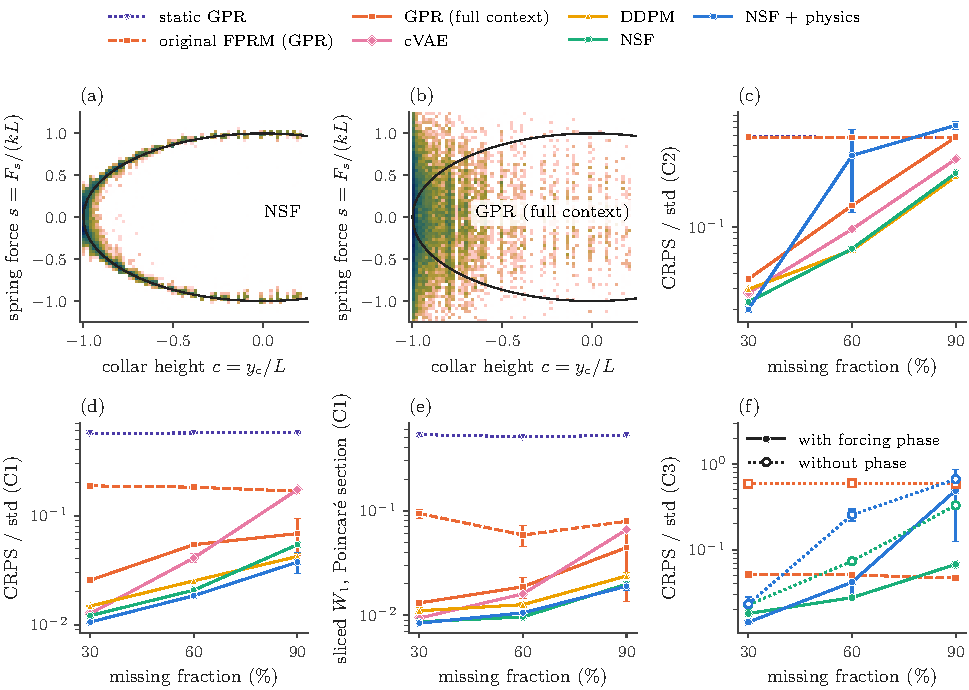
\includegraphics[width=\textwidth]{figures/fig_fprm.pdf}
\caption{Reconstruction scores versus missing fraction. (a) NSF and (b) GPR (full context): posterior samples of the spring force $s$ versus the complete collar height $c$ for the missing entries of C2 at $90\%$ missing data that have no observed neighbor (first random mask; logarithmic color scale); the flow places its samples on both branches $s=\pm(1-c^{2})^{1/2}$ (black), whereas the GPR averages them. (c) CRPS versus the missing fraction for C2. (d) CRPS and (e) sliced Wasserstein distance between imputed and true Poincar\'e sections for C1. (f) CRPS for C3 with (filled markers) and without (open markers, dotted lines) the forcing phase; the original FPRM receives the phase in the first variant. Markers show the mean over two random masks and bars the half-range; the CRPS is normalized by the standard deviation of the target.}
\label{fig:fprm}
\end{figure*}

Table~\ref{tab:fprm} lists all metrics at $90\%$ missing data, the most demanding setting, and Fig.~\ref{fig:fprm} shows how the scores depend on the missing fraction. The results are presented in the order dictated by the identifiability analysis: a trivial control, an identifiable task, a task made ambiguous by symmetry, and its driven analogue, in which the forcing phase can lift the ambiguity.

\subsection{A trivial control (C0)}\label{sec:res_c0}

With the angle complete, a Savitzky--Golay derivative (window of 11 samples, degree 4) reconstructs the angular velocity with $\rho=0.9997$ and $\mathrm{NRMSE}=0.023$--$0.025$ at every missing fraction, since it never uses the incomplete channel. The flow, trained only on the observed pairs and conditioned on the full vector of Eq.~\eqref{eq:context}, is less accurate: $\rho=0.998$ at $30\%$ and $0.65$ at $90\%$ missing data. Its input is the unwrapped angle, whose secular drift during rotations makes it a poor observable for delay reconstruction and inflates the selected delay ($\tau=26$ samples). Reconstruction from the angle is therefore not a meaningful benchmark, and the tasks below use observables that are not related by differentiation.

\subsection{Identifiable chaotic dynamics (C1)}\label{sec:res_c1}

When the spring force is complete, the magnitude $|c|=(1-s^{2})^{1/2}$ follows from the holonomic identity, and the informative targets are the branch, i.e., the sign of $\cos\theta$, and the angular velocity. Every imputer that receives the full conditioning vector reconstructs $(c,\dot\theta)$ accurately at $30\%$ missing data ($\rho\ge0.994$), and the differences emerge as data are removed [Fig.~\ref{fig:fprm}(d)]. The original FPRM, which relies on the delay window alone, remains at $\rho\approx0.87$--$0.89$ and $\mathrm{NRMSE}\approx0.45$--$0.49$ at all fractions.

The accuracy of the original FPRM is limited not by identifiability, which holds for this task [Fig.~\ref{fig:fprm_scheme}(b)], but by the number of training points. A nearest-neighbor predictor on the same delay window reaches $\rho=0.98$ at $30\%$ missing data when all $2.8\times10^{4}$ observed entries serve as its library, but only $\rho=0.84$ when the library is restricted to 1200 points, the size of the training set of the Gaussian process. Resolving a folded chaotic attractor from a delay window alone requires a dense library, as in convergent cross mapping~\cite{Sugihara2012}. Fitting the same Gaussian process to all labeled samples at $90\%$ missing data (about 3900--4000 per mask) confirms this diagnosis: its correlation rises to $\rho=0.936$ and its CRPS falls from $0.167$ to $0.112$, with a coverage of $0.93$.

Among the purely data-driven engines that receive the full conditioning vector, the flow and the cVAE are on par at $30\%$ (CRPS $0.012$ and $0.013$), the flow is best at $60\%$ ($0.021$), and at $90\%$ the diffusion model is better ($0.042$ against $0.054$), more accurate in the median (NRMSE $0.135$ against $0.189$), and better calibrated (coverage $0.93$ against $0.80$). The physics-regularized flow attains the lowest CRPS at every fraction ($0.011$, $0.018$, and $0.037$, that is, $13\%$, $11\%$, and $31\%$ below the unregularized flow), and at $90\%$ it reduces the fraction of samples on the wrong branch from $4.7\%$ to $2.7\%$. Against the original FPRM, its CRPS is $4.5$ times lower at $90\%$ missing data ($3.6$ and $5.7$ times for the two masks), and still three times lower ($2.5$ and $3.7$ times) when the Gaussian process is trained on every label. The GPR that receives the same full conditioning vector closes much of this gap (CRPS $0.068$), which shows that a large part of the gain comes from the conditioning information, i.e., from the observed neighbors and the forcing phase, rather than from the density model alone. The price of the physics term is calibration: the coverage of the nominal $90\%$ intervals falls to $0.66$, so that the regularized flow is overconfident.

The benefit becomes tangible when the dynamics itself is reconstructed. In Fig.~\ref{fig:reconstruction}, every missing entry of an eight-period window at $90\%$ missing data, 236 entries of each target, is imputed with the regularized flow and with the original FPRM. The posterior medians of the flow follow the continuous trajectory through rapid rotations and slow librations, with root-mean-square errors of $0.22$ in $c$ and $0.17$ in $\dot\theta\sqrt{L/g}$, against $0.34$ and $0.45$ for the original FPRM, whose Gaussian means scatter between the branches. Imputing $(c,\dot\theta)$ at all 1137 missing section points and combining them with the noise-free spring force rebuilds the Poincar\'e section. The flow recovers the folded, fractal structure of the attractor ($W_1=0.023$), whereas the original FPRM smears it into a diffuse cloud ($W_1=0.063$). On the benchmark, whose section is taken one sample later, at $\Omega t=2\pi/32$, because its sampled record starts one sample after a forcing period, both flows produce the sections closest to the true one ($W_1=0.019$--$0.020$ at $90\%$, against $0.024$ for the diffusion model and $0.079$ for the original FPRM) [Fig.~\ref{fig:fprm}(e)].

\begin{figure*}
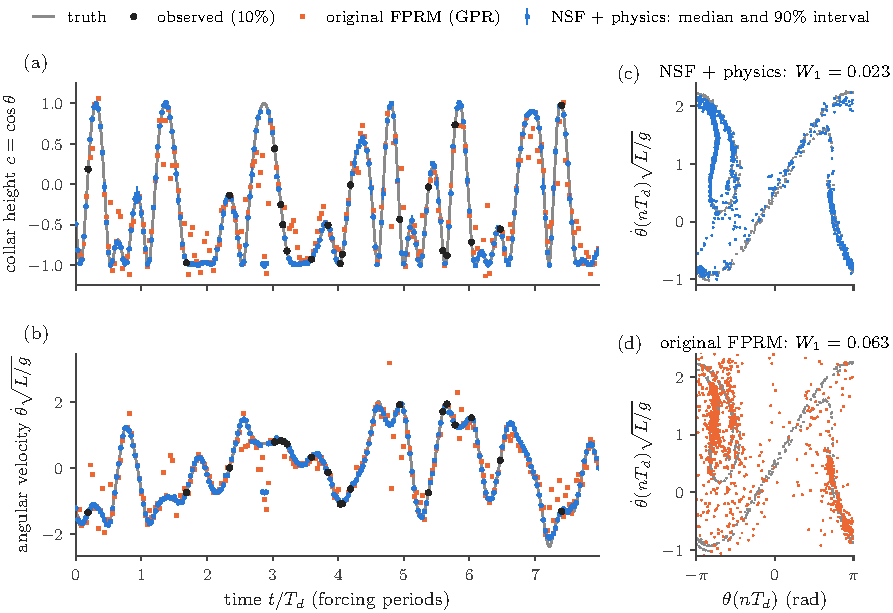
\includegraphics[width=\textwidth]{figures/fig_reconstruction.pdf}
\caption{Chaotic dynamics recovered from $10\%$ of the collar-height and angular-velocity records (task C1, first random mask). (a) Collar height and (b) angular velocity over eight forcing periods: continuous true trajectory (gray line), observed samples (black dots), posterior median and central $90\%$ interval of the physics-regularized flow at every missing sample (blue), and Gaussian mean of the original FPRM (orange squares). (c) Physics-regularized flow and (d) original FPRM: stroboscopic Poincar\'e section at the phase $\Omega t=0$ of the drive, rebuilt at the 1137 missing section points from the noise-free spring force and one imputation of $(c,\dot\theta)$ (colored), over the true section (gray); $W_1$ is the sliced Wasserstein distance in $(s,c,\dot\theta)$.}
\label{fig:reconstruction}
\end{figure*}

\subsection{Symmetry-induced ambiguity (C2)}\label{sec:res_c2}

When the collar height is complete, the original FPRM returns $\rho\approx0$ at every missing fraction, as predicted by the reflection symmetry, and its CRPS does not improve as data are added [Fig.~\ref{fig:fprm}(c)]. At $30\%$ missing data the observed neighbors resolve the sign for almost every entry, all imputers that receive the full conditioning vector succeed ($\rho\ge0.994$), and the two flows have the lowest errors (NRMSE $0.074$; CRPS $0.023$ without and $0.020$ with the physics term). At $90\%$, about half of the missing entries ($0.9^{6}\approx53\%$ expected) have no observed neighbor within three samples, and their exact conditional distribution is bimodal. The flow represents both branches [Fig.~\ref{fig:fprm}(a)], whereas the GPR with the full conditioning vector, whose marginal-likelihood optimization (with a single start) converges to a noise-dominated solution, returns a broad Gaussian centered at zero [Fig.~\ref{fig:fprm}(b)]. The CRPS values of the flow and of the diffusion model ($0.29$ and $0.27$) are about half that of the GPR ($0.58$). In this regime the correlation of the posterior median is a misleading score, because the median of a nearly symmetric bimodal distribution lies between the branches: the cVAE, whose Gaussian decoder tends to merge the branches, reaches a higher correlation ($0.63$) but a worse CRPS ($0.38$).

\subsection{The forcing phase restores identifiability (C3)}\label{sec:res_c3}

In this task the original FPRM, with and without the phase appended to its delay window, is compared with the two flows. In the driven system the phase lifts the ambiguity [Fig.~\ref{fig:fprm}(f)], as anticipated by the cross-mapping test of Fig.~\ref{fig:fprm_scheme}(d). With the phase, the original FPRM reconstructs $s$ with $\rho=0.989$ and CRPS $0.047$ at $90\%$ missing data, better than the flow ($\rho=0.975$, CRPS $0.067$), whose conditional density is harder to estimate from about 4000 labeled samples; at $30\%$ and $60\%$ the flow is more accurate (NRMSE $0.069$ and $0.090$, against $0.163$ and $0.160$). Without the phase, the original FPRM fails completely ($\rho\approx0$), and the flow, which then relies on the observed neighbors alone, falls from $\rho=0.993$ at $30\%$ to $0.43$ at $90\%$.

\subsection{When the physics helps and when it hurts}\label{sec:res_physics}

At $30\%$ missing data the physics residuals lower the CRPS of the flow in C1, C2, and C3 with the phase (by $13\%$, $14\%$, and $21\%$, respectively) and change it by less than $2\%$ in C3 without the phase; at this fraction the observed neighbors resolve the branch of most entries, and the residuals act only as a mild regularizer of the density. At larger missing fractions they continue to help in C1, where the gravitational and forcing terms of Eq.~\eqref{eq:res_eom} discriminate the sign of $\cos\theta$ and the kinematic relation fixes the angular velocity, but they are harmful in C2 and C3. At $90\%$ missing data the regularized flow attains only $\rho=0.03$ in C2 and $0.35$ in C3 without the phase, against $0.49$ and $0.43$ for the unregularized flow, and its coverage drops to $0.59$ and $0.38$; in C2 one mask collapses already at $60\%$ ($\rho=-0.04$). The same failure appears in C3 with the phase, where the target is identifiable: at $60$--$90\%$ the CRPS is worse than without the physics term in three of the four runs, and one mask collapses at $90\%$ ($\rho=0.05$, against $0.98$ without the physics term).

The pattern follows from the structure of the residuals. Where the target is ambiguous, the residuals are nearly invariant under $\hat s\to-\hat s$ and cannot select a branch, but they penalize the probability that a flow with a unimodal base must place between the two branches~\cite{Cornish2020}. The flow can lower this penalty by collapsing onto one branch, after which it assigns high confidence to a single, often wrong, sign. In C3, moreover, the only sign-discriminating term of Eq.~\eqref{eq:res_c3}, $f(t)\,\hat s^{3}$, competes with the noise that the numerical second derivative contributes to the residual, $\hat s^{2}\,\delta\ddot c$, where $\delta\ddot c\approx0.107$ is the standard deviation of the Savitzky--Golay estimate of $\ddot c$ for a measurement noise of $0.01$. As an order-of-magnitude estimate, the discriminating term falls below this noise whenever $A|\hat s\cos\Omega t|<\delta\ddot c$, i.e., $|\hat s\cos\Omega t|<0.13$, which is the case for $24\%$ of the samples on the attractor; the residual is therefore poorly conditioned even when the phase is available. The collapse also escapes early stopping, because the validation likelihood is computed on labeled entries and does not see the imputations of unlabeled ones. These observations are related to the known failure modes of physics-informed training, in which soft constraints make the loss landscape ill conditioned~\cite{Krishnapriyan2021,WangTengPerdikaris2021}; here, in addition, the residual carries no information about the branch.

\subsection{Flow versus diffusion model}\label{sec:res_engine}

The diffusion model is the strongest competitor of the flow, and the choice between the two engines rests on the following evidence. Without physical residuals neither engine dominates: the flow attains a lower CRPS than the DDPM at $30\%$ and $60\%$ missing data in task C1 (by $18\%$) and at $30\%$ in task C2 (by $22\%$), the DDPM attains a lower CRPS at $90\%$ (by $22\%$ in C1 and $6\%$ in C2), and the two agree to within $3\%$ at $60\%$ in C2; each strict ranking holds for both masks. The DDPM reached its lowest validation loss within the last $10\%$ of its 6000 training steps in every run, so that its scores might still improve slightly with a longer budget. The intervals of the DDPM are conservative (coverage $0.93$--$0.97$ in C1), whereas those of the flow become too narrow as data are removed ($0.80$ at $90\%$); the flow, however, reproduces the invariant measure more faithfully at every missing fraction, with sliced distances on the Poincar\'e section smaller by $16$--$24\%$.

The decisive differences are structural. With the architectures of Table~\ref{tab:hyper} on one processor thread, drawing 64 samples for 1500 missing entries of task C1 took $1.8$~s with the flow and $47$~s with the DDPM, because the flow evaluates its conditioner six times per sample (two autoregressive passes in each of three transforms), whereas the DDPM evaluates its denoiser once per noise level, i.e., 100 times. For the scalar target of task C2, whose spline parameters depend only on the conditioning vector and are computed once per entry, the ratio reaches three orders of magnitude ($0.02$~s against $27$~s). Accelerated samplers reduce the number of denoising steps at some cost in sample quality~\cite{SongMengErmon2021}, which narrows this gap without closing it.

A physics-regularized training step needs gradients through the samples: the flow obtains them from one reparameterized pass, whereas the DDPM requires backpropagation through its entire reverse chain, which multiplied the cost of differentiating a penalty evaluated on the samples by more than $30$ in task C1 and by more than $200$ in task C2 (Table~S8 of the supplementary material). Physics-informed diffusion models avoid this cost by evaluating the residuals on the denoised mean estimate at each training noise level, or on a few accelerated sampling steps, rather than on full-chain samples of the model~\cite{Bastek2025}. Moreover, the exact likelihood of a diffusion model requires the integration of a probability-flow ordinary differential equation~\cite{Song2021}, whereas the flow returns it directly. Residuals evaluated on samples of the model, as in Eq.~\eqref{eq:loss}, were therefore affordable only for the flow, and the physics-regularized flow attains the lowest mean CRPS of all imputers in task C1 at every missing fraction: $27$--$29\%$ below that of the DDPM at $30\%$ and $60\%$ missing data ($25$--$31\%$ for the individual masks), and $11\%$ below at $90\%$, where the two masks disagree (CRPS $0.0454$ and $0.0295$, against $0.0447$ and $0.0395$ for the DDPM). The price is calibration: every flow in this study covered less than the nominal $90\%$, the regularized ones even less, a deficit that must be removed, for instance by recalibration on held-out entries~\cite{Kuleshov2018}, before the intervals are used.

\section{Interactive computational laboratory}\label{sec:lab}

\begin{figure*}
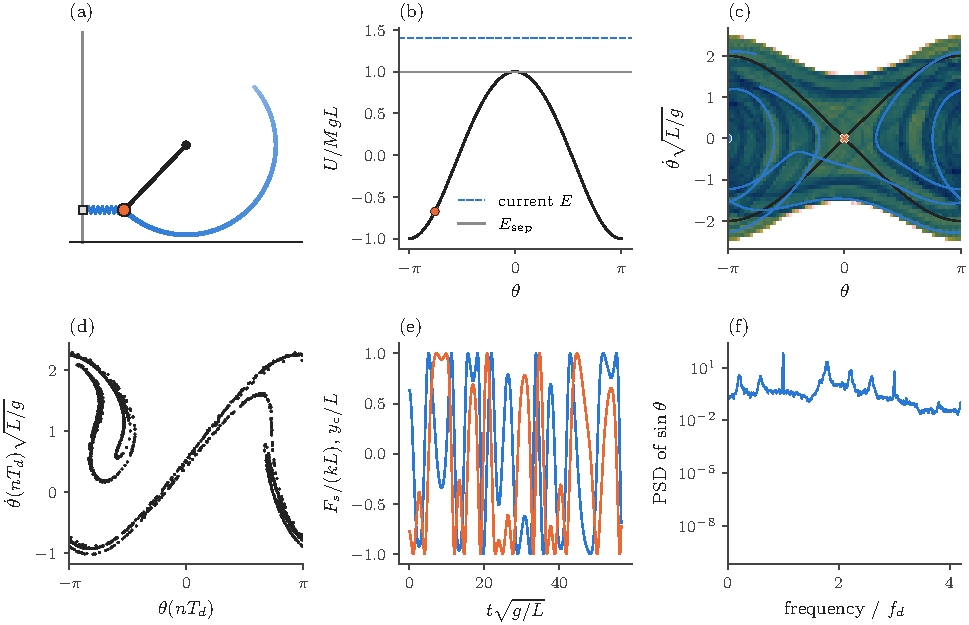
\includegraphics[width=\textwidth]{figures/fig_dashboard.pdf}
\caption{Snapshot of the interactive laboratory for the chaotic reference state ($\mu=-0.8$, $\gamma=0.25$, $A=0.8$, $\Omega=2/3$). (a) Schematic with the fading motion trail of the mass, drawn through the Hermite interpolant. (b) Energy landscape with the separatrix energy and the current energy. (c) Phase portrait: logarithmic occupation histogram, separatrix of the unforced system (black), recent trajectory, and equilibria of the unforced system. (d) Stroboscopic Poincar\'e section. (e) Normalized spring force $F_s/(kL)$ (blue) and collar height $y_c/L$ (orange). (f) Power spectral density of the spring force as a function of frequency in units of the drive frequency $f_d=\Omega/(2\pi)$.}
\label{fig:dashboard}
\end{figure*}

Every result of this article is produced by an open laboratory written in Python. The package \texttt{piar} contains one module per layer of the analysis: \texttt{physics} (the model, its closed-form invariants, and compiled right-hand sides), \texttt{integrators} (a compiled DOP853, velocity Verlet, fourth-order Runge--Kutta, and exact periods), \texttt{chaos} (stroboscopic maps, continuation, Lyapunov spectra, Floquet multipliers, Feigenbaum cascades, Melnikov integrals, and correlation sums), \texttt{stochastic} (BAOAB Langevin dynamics), \texttt{embedding} (average mutual information and false nearest neighbors), \texttt{fprm} (conditioning vectors, conditional flows, cVAE, DDPM, Gaussian processes, physics residuals, and metrics), \texttt{smooth} (rendering of trajectories), and \texttt{dashboard}. Array operations rely on NumPy~\cite{Harris2020} and SciPy~\cite{Virtanen2020}, numerical kernels are compiled with Numba~\cite{Lam2015}, the neural networks are implemented in PyTorch~\cite{Paszke2019}, the flows are provided by \texttt{zuko}~\cite{zuko}, the Gaussian processes by scikit-learn~\cite{Pedregosa2011}, and the figures are drawn with Matplotlib~\cite{Hunter2007}.

Trajectories are rendered from continuous representations of the solution. Conservative trajectories are drawn from the dense output of DOP853 (Sec.~\ref{sec:cases_method}). For fixed-step integration, the integrator provides $\theta$ and $\dot\theta$ at each grid point and the equation of motion provides $\ddot\theta$ at the cost of one evaluation per stored point, so that each interval is filled with the cubic Hermite interpolants of $\theta$ and $\dot\theta$, which are continuously differentiable and accurate to fourth order in the step~\cite{HairerNW1993}; this is how the driven trajectories of Figs.~\ref{fig:attractor}(a) and \ref{fig:reconstruction} are drawn. Angles are wrapped onto the cylinder with explicit breaks at the cut $\theta=\pm\pi$, so that rotations are not crossed by spurious horizontal segments.

The interactive part of the laboratory follows the environments long used in physics teaching, such as Easy Java Simulations~\cite{Esquembre2004} and the Open Source Physics project~\cite{Christian2011}. The interactive dashboard (Fig.~\ref{fig:dashboard}) is a Jupyter notebook in which sliders for $(\mu,\gamma,A,\Omega)$ and for the initial condition drive six linked panels: a schematic with a fading motion trail, the energy landscape with the current energy, the phase portrait, the stroboscopic Poincar\'e section, the two measurable observables, and the power spectrum of the spring force. The notebook also draws the four diagnostics of Fig.~\ref{fig:cases} for any case and animates the pendulum and its phase-space trajectory from the same Hermite interpolant. A browser-based version, written in JavaScript and requiring no installation, reproduces the five cases of Table~\ref{tab:cases} and the chaotic reference state; it integrates the equation of motion with fourth-order Runge--Kutta at a step of $2\times10^{-3}\,t_c$, keeps the energy of the conservative cases constant to better than $10^{-10}\,MgL$ over 100~s, stores every step in the motion trail, and updates the four diagnostics in real time.

All figures follow a common style: Computer Modern typography rendered by \LaTeX, axes without top and right spines, and perceptually uniform scientific colormaps that remain legible under color-vision deficiency (\textit{batlow} for magnitudes and \textit{vik} for signed quantities~\cite{Crameri2020}), together with a categorical palette whose adjacent pairs were checked for separability under simulated color-vision deficiency. Eight experiment scripts and five figure scripts regenerate every figure and number from fixed random seeds and write the numerical results to JSON files. Unit tests check the closed-form invariants, the agreement of the compiled DOP853 with SciPy, the second-order convergence of velocity Verlet, the exact periods, the determinant of the Poincar\'e map, the Lyapunov sum rule, the pendulum limit of the Melnikov integrals, and the accuracy of the Hermite rendering.

\paragraph*{Use of generative artificial intelligence.} A generative artificial-intelligence tool, Claude (model Claude Opus 5.5; Anthropic PBC, San Francisco, CA, USA), accessed through the Claude application in September 2026, was used in three parts of this work: (i) writing and debugging the analysis code, namely the \texttt{piar} package, the experiment and figure scripts, the unit tests, the notebook, and the browser-based simulation; (ii) running the numerical experiments and documenting their settings and outputs; and (iii) drafting and editing the manuscript. The tool was used to accelerate software development, testing, and documentation. Because this use could affect the findings, every figure and number reported in this article is regenerated by the released code from fixed random seeds, the unit tests check the closed-form invariants, the integrators, and the chaos diagnostics against analytical or independent results, and the bibliographic data of every reference were checked against publisher or index records. The author takes full responsibility for the code, the numerical results, and the text.

\section{Discussion}\label{sec:discussion}

\subsection{Symmetry decides what can be reconstructed}

The reconstruction tasks were designed from the symmetry of the model rather than from the capacity of the learners, and the outcome is correspondingly sharp. Delay coordinates of the collar height cannot determine the sign of the spring force, because the reflection $\theta\to-\theta$ leaves the collar height invariant, and the original FPRM, which regresses on delay coordinates alone, therefore returns the average of the two branches, with a correlation near zero ($|\rho|<0.05$) at every missing fraction. This is an instance of a general principle of observability theory: the quality of a reconstruction depends on the observable, and symmetries can render an observable blind to part of the state~\cite{LetellierAguirre2002,Letellier2005}. The FPRM inherits this constraint from Takens' theorem, and the cross-mapping test of Fig.~\ref{fig:fprm_scheme} offers a cheap way to detect it before any model is trained. Two pieces of information restore identifiability in the PIAR: the observed neighbors of the incomplete channel, through continuity, and the phase of the forcing, which distinguishes mirror states of the driven system. A practical rule follows for the design of sensor layouts: a channel that is invariant under a symmetry of the dynamics should not be the only complete record for a channel that the symmetry changes, unless another signal, such as a drive or a reference clock, resolves that ambiguity.

\subsection{Distributions rather than points}

When the ambiguity is genuine, a conditional generative model is the appropriate tool, because it represents the branches instead of averaging them. Point metrics computed on the posterior median can then misrank reconstructions, as the higher correlation but worse CRPS of the cVAE in task C2 illustrates, and proper scoring rules~\cite{Gneiting2007}, together with the fraction of samples on the correct branch, are the relevant measures. Distributional fidelity also matters downstream: the invariant measure of the attractor, probed here through the Poincar\'e section, is recovered by the flow and blurred by the original FPRM (Fig.~\ref{fig:reconstruction}). The choice of engine can therefore be guided by the cross-mapping test. When the test reveals a mirror branch, a conditional generative model is required, unless observed neighbors resolve the branch, as in task C2 at small missing fractions. When the test indicates identifiability, a Gaussian process on an informative input is a strong and inexpensive baseline, provided that its training set resolves the folded attractor, as in task C3 with the phase but not in task C1; the nearest-neighbor library test of Sec.~\ref{sec:res_c1} checks this condition at negligible cost. Among generative models, a flow is preferable when physical residuals are to be imposed or many samples are required, and a diffusion model when labels are scarce and no residuals are imposed, or when conservative intervals matter more than computational cost (Sec.~\ref{sec:res_engine}).

\subsection{Physics as a double-edged sword}

Equation-of-motion residuals helped exactly where they carried information about the unknown degree of freedom: in task C1, the gravitational and forcing terms discriminate the sign of $\cos\theta$, and the kinematic relation fixes the angular velocity. Where the residuals were nearly invariant under the ambiguity, or dominated by the noise of numerical derivatives, they did not add information about the branch and, at $60$--$90\%$ missing data, pushed the flow to collapse onto a single branch. Three practical rules follow: a residual should be imposed only when it is informative about the ambiguous degree of freedom and well conditioned with respect to the noise of its derivatives; regularized models should be validated on imputations of artificially masked observed entries rather than on the likelihood of labeled ones; and sharpened posteriors must be checked for calibration (Sec.~\ref{sec:res_engine}). The topological origin of the collapse suggests remedies that preserve multimodality by construction: mixture base distributions, continuously indexed flows~\cite{Cornish2020}, and flows defined on the circle~\cite{Rezende2020}, which respect the periodicity of the angle. Structure-preserving models offer a complementary route to physical consistency. Hamiltonian and Lagrangian networks~\cite{Greydanus2019,Cranmer2020} and their dissipative extensions~\cite{Sosanya2022} could supply the dynamical prior of a future FPRM through the architecture rather than through the loss; the Hamiltonians learned by generic networks are not separable, and explicit symplectic integrators for nonseparable Hamiltonians~\cite{Tao2016} would then be needed to roll them out.

\subsection{Limitations and outlook}

The study is confined to a single degree of freedom, to a single chaotic reference state, to a harmonic torque rather than to the multiplicative base excitation of real isolators, and to synthetic data with missing-completely-at-random masks and a fixed noise level; gaps that are correlated in time, or caused by saturation, would require the missingness mechanism to be modeled~\cite{LittleRubin2019}. The benchmark uses two random masks per setting, which suffices to separate the qualitative regimes reported here but not to rank imputers whose scores differ by a few percent. The original FPRM was reimplemented with an exact Gaussian process; scalable approximations would allow it to use every labeled row at small missing fractions.

Several extensions follow naturally. An experimental PIAR instrumented with a load cell and a linear encoder would test the framework on real sensor records, and chains of coupled pendulums, in which one site is fully observed, would test it in higher dimension. Reconstructed records could also feed system identification, from the sparse regression of governing equations~\cite{Brunton2016} to the Bayesian estimation of physical parameters. For the latter, spectral Whittle likelihoods~\cite{Whittle1953,Sykulski2019} can be sampled with ensemble Markov chain Monte Carlo~\cite{GoodmanWeare2010,ForemanMackey2013} or with nested sampling~\cite{Skilling2006,Speagle2020}, which also yields the evidence for comparing competing models through Bayes factors~\cite{KassRaftery1995}, and the calibration of the resulting posteriors can be checked by simulation-based calibration~\cite{Talts2018}. Propagating the imputation uncertainty of the flow into such inferences by multiple imputation~\cite{LittleRubin2019} is a direct benefit of a generative engine that a point regressor cannot provide.

Finally, the same laboratory can be used in teaching. The five conservative regimes illustrate the classification of orbits by energy, the degenerate critical point, and the lengthening of the period predicted by the normal form; the driven system displays the Feigenbaum cascade, the Melnikov mechanism, and a strange attractor; and the FPRM turns Takens' theorem into a concrete, testable computation. Because every figure and number can be regenerated, the PIAR can accompany a course from analytical mechanics to data-driven dynamics.

\section{Conclusions}\label{sec:conclusions}

The spring-coupled inverted pendulum has been developed into a transparent benchmark for the recovery of missing dynamics and used to extend the full--partial reconstruction mapping with a generative engine. Five conclusions emerge.

First, the conservative dynamics is governed by the single parameter $\mu=kL/(Mg)-1$, which unfolds a subcritical pitchfork at $\mu=0$. Near this critical point the resonance frequency and the tilt of the saddles vanish as $\mu^{1/2}$ but the barrier vanishes as $\mu^{2}$, which quantifies the trade-off between isolation and robustness that governs inverted-pendulum isolators. Five canonical regimes, computed with trajectories that conserve energy to $10^{-10}\,MgL$ and periods that agree with exact quadratures, display a libration inside the upright well, whose period is lengthened by $4.2\%$, in agreement with the $4.1\%$ predicted by the normal form; critical slowing down at the degenerate point; and rotations near and far from the separatrix.

Second, under damping and forcing the separatrix splits and seeds chaos: no chaotic state was found below the Melnikov threshold curve $A_c(\Omega)$, which gives $(A/\gamma)_c=2.049$ at the reference drive frequency, and the dynamics reaches, through a period-doubling cascade with ratios converging to Feigenbaum's constant, a strange attractor with $\lambda_1=0.0956\,(g/L)^{1/2}$ and $D_{\mathrm{KY}}=2.277$, whose dimension is consistent with the embedding dimension $d_E=5$ selected by false nearest neighbors.

Third, symmetry decides what can be reconstructed. A model-free cross-mapping test shows that the collar height is recoverable from the spring force ($\rho=0.99$) but not conversely ($\rho=-0.01$), because of the reflection $\theta\to-\theta$, and that the phase of the forcing restores identifiability ($\rho=0.99$). The mechanism is generic: a complete channel that is invariant under a symmetry of the dynamics, such as the $z$ variable of the Lorenz system under $(x,y)\to(-x,-y)$, cannot by itself identify a variable that the symmetry changes~\cite{LetellierAguirre2002}, and the same test detects the problem before any model is trained.

Fourth, recast as conditional density estimation with a neural spline flow, the FPRM gains most from its conditioning information and from its ability to represent several branches. With the spring force observed and $90\%$ of the collar-height and angular-velocity records missing, the physics-regularized flow lowers the continuous ranked probability score by a factor of 4.5 relative to the reimplemented original FPRM, by a factor of 3 when the latter is trained on every labeled sample, and by a factor of 1.8 relative to a Gaussian process with the same conditioning vector; it also recovers the fractal Poincar\'e section; when the target is ambiguous, the flow preserves both branches while regression averages them. At large missing fractions, physical residuals, holonomic or dynamical, help only when they are informative about the ambiguous degree of freedom and well conditioned; otherwise they can induce mode collapse.

Fifth, the complete study is available as an open laboratory, with a Python package, an interactive dashboard, and a browser-based simulation, in which every figure and number is regenerated from fixed seeds. Because its predictions can be checked against exact mechanics, the PIAR offers a controlled setting in which new reconstruction engines, physical priors, and sensor layouts can be tested before they are deployed on the incomplete records of real mechanical systems.


\section*{Supplementary Material}
See the supplementary material for the complete benchmark tables of every task, missing fraction, and random mask; the embedding parameters of the four tasks and the diagnostics of Secs.~\ref{sec:res_c1} and \ref{sec:res_physics}; the cost and symmetry checks of Secs.~\ref{sec:res_engine} and \ref{sec:attractor}; the diagnostic figures of the five conservative regimes at full size; and a guide to the laboratory that relates every figure and table to the script that produces it.

\begin{acknowledgments}
The use of a generative artificial-intelligence tool in code development, numerical experiments, and manuscript preparation is described in Sec.~\ref{sec:lab}.

\end{acknowledgments}

\section*{Author Declarations}
\subsection*{Conflict of Interest}
The author has no conflicts to disclose.

\subsection*{Author Contributions}
\textbf{Fredy Alexander Orjuela L\'opez:} Conceptualization (lead); Methodology (lead); Software (lead); Formal analysis (lead); Investigation (lead); Visualization (lead); Writing -- original draft (lead); Writing -- review \& editing (lead).

\section*{Data Availability Statement}
The data that support the findings of this study are available within the article and its supplementary material. The code and data that regenerate every figure and number (the \texttt{piar} package, the experiment and figure scripts, the unit tests, the interactive notebook, the browser-based simulation, and the numerical results) are openly available in GitHub at \url{https://github.com/faorjuelal/PIAR}.
\ifdefempty{\zenodoDOI}{%
An archived version will be deposited in Zenodo upon publication.%
}{%
An archived version is openly available in Zenodo at \url{https://doi.org/\zenodoDOI}.%
}

\appendix
\section{Derivations}\label{app:derivations}

\subsection{Separatrix energy and barrier}

For $\mu>0$, Eq.~\eqref{eq:thetastar} gives $\cos\theta^{*}=(1+\mu)^{-1}$ and $\sin^{2}\theta^{*}=1-(1+\mu)^{-2}$. Substituting into Eq.~\eqref{eq:U}, with $kL^{2}=MgL(1+\mu)$, gives
\begin{equation}
\begin{split}
U(\theta^{*}) &= MgL\left[\frac{1}{1+\mu}+\frac{1+\mu}{2}-\frac{1}{2(1+\mu)}\right]\\
&= MgL\,\frac{(1+\mu)^{2}+1}{2(1+\mu)},
\end{split}
\end{equation}
which is Eq.~\eqref{eq:Esep}; subtracting $U(0)=MgL$ yields the barrier of Eq.~\eqref{eq:barrier}. The curvature at the saddle, $U''(\theta^{*})=MgL[(1+\mu)^{-1}-(1+\mu)]=-MgL\,\mu(2+\mu)/(1+\mu)$, gives the growth rate $\nu_*=[(g/L)\,\mu(2+\mu)/(1+\mu)]^{1/2}$ with which trajectories leave the tilted saddles.

\subsection{Normal form and amplitude-dependent frequency}

With $\sin\theta=\theta-\theta^{3}/6+O(\theta^{5})$ and $1-(1+\mu)\cos\theta=-\mu+(1+\mu)\theta^{2}/2+O(\theta^{4})$, the product in Eq.~\eqref{eq:eom_dimless} becomes $-\mu\theta+\bigl[\tfrac12(1+\mu)+\tfrac16\mu\bigr]\theta^{3}+O(\theta^{5})$, which is Eq.~\eqref{eq:normal_form}. At $\mu=0$ the potential reduces to $U/MgL=\cos\theta+\tfrac12\sin^{2}\theta=1-\theta^{4}/8+O(\theta^{6})$. For $\mu>0$, Eq.~\eqref{eq:normal_form} is a softening Duffing oscillator, $\theta''+\mu\theta-b\,\theta^{3}=0$ with $b=(3+4\mu)/6$. The Lindstedt--Poincar\'e expansion of a periodic solution of amplitude $a$ gives, in natural units, $\omega^{2}=\mu-\tfrac34\,b\,a^{2}+O(a^{4})$~\cite{Strogatz2015}, hence
\begin{equation}
\frac{\omega}{\omega_0} = 1-\frac{3b\,a^{2}}{8\mu}+O(a^{4}) = 1-\frac{(3+4\mu)\,a^{2}}{16\,\mu}+O(a^{4}),
\end{equation}
which is Eq.~\eqref{eq:lindstedt}. For case 2 ($\mu=0.5$, $a=0.2516$~rad) the predicted frequency shift is $3.96\%$, against the exact $4.00\%$ obtained from the period $16.0323$~s and $2\pi/\omega_0=15.3906$~s; in terms of the period, the lengthening is $4.12\%$ predicted and $4.17\%$ exact, and the difference is of the order of the neglected $O(a^{4})$ terms.

\subsection{Exact periods}

With the energy per unit inertia, $\epsilon=E/(ML^{2})$, and $\upsilon(\theta)=U(\theta)/(ML^{2})$, the period of Eq.~\eqref{eq:period} reads $T=\oint\mathrm d\theta\,\{2[\epsilon-\upsilon(\theta)]\}^{-1/2}$. For a libration symmetric about a center $\theta_e$ ($\theta_e=0$ in the upright well, $\theta_e=\pi$ in the hanging well) with turning points $\theta_e\pm a$, the substitution $\theta=\theta_e+a\sin\xi$ removes the inverse-square-root singularity at the turning points,
\begin{equation}
T = 4\int_0^{\pi/2}\frac{a\cos\xi\,\mathrm d\xi}{\{2[\epsilon-\upsilon(\theta_e+a\sin\xi)]\}^{1/2}},
\end{equation}
and the resulting smooth integral was evaluated by adaptive quadrature with a relative tolerance of $10^{-12}$; the amplitude $a$ was found by bracketing the root of $\upsilon(\theta_e+a)=\epsilon$. For rotations the integrand is regular over one revolution. Near a hyperbolic saddle with growth rate $\nu$, the velocity vanishes linearly with the distance to the saddle, so that the time spent in its neighborhood diverges as $\nu^{-1}\ln(MgL/|E-E_{\mathrm{sep}}|)$ per saddle passage as $E\to E_{\mathrm{sep}}$; the period contains one or two such passages. At the degenerate point $\mu=0$, where $\upsilon\simeq(g/L)(1-\theta^{4}/8)$ near the top, the substitution $\theta=[8|\epsilon-g/L|L/g]^{1/4}\eta$ shows instead that the passage time scales as $|E-E_{\mathrm{sep}}|^{-1/4}$.

\subsection{Melnikov integrals}

For $\mu<0$ and per unit inertia, the homoclinic orbit of the upright saddle has $\epsilon=1$ in natural units. With $\chi=2\pi-\theta$, the angular distance to the saddle for $\theta\in[\pi,2\pi]$, energy conservation gives
\begin{equation}
\dot\theta_h^{2} = 4\sin^{2}\frac{\chi}{2}-\kappa\sin^{2}\chi = 4\sin^{2}\frac{\chi}{2}\left[1-\kappa\cos^{2}\frac{\chi}{2}\right],
\end{equation}
a form free of the cancellation in $1-\cos\theta$ near the saddle. With $\Lambda=(1-\kappa)^{1/2}$ and time measured from the bottom of the loop, the orbit is
\begin{equation}
\dot\theta_h(t) = \frac{2\Lambda^{2}\,\mathrm{sech}(\Lambda t)}{1-\kappa\,\mathrm{sech}^{2}(\Lambda t)},
\end{equation}
whose integral is $\sin[(\theta_h-\pi)/2]=\tanh(\Lambda t)/[1-\kappa\,\mathrm{sech}^{2}(\Lambda t)]^{1/2}$. The substitution $u=\cos(\chi/2)$ turns $I_0=\oint\dot\theta_h\,\mathrm d\theta$ into $8\int_0^1(1-\kappa u^{2})^{1/2}\,\mathrm du$, and $I_1$ follows from the residues of its integrand at the poles $\Lambda t=i(\pi/2\pm\arcsin\sqrt\kappa)$ of $\dot\theta_h$. The integrals of Eq.~\eqref{eq:melnikov_integrals} evaluate to
\begin{align}
I_0 &= 4\left[\Lambda+\frac{\arcsin\sqrt\kappa}{\sqrt\kappa}\right],\\
I_1(\Omega) &= 2\pi\,\frac{\cosh\bigl(\Omega\arcsin\sqrt\kappa/\Lambda\bigr)}{\cosh\bigl[\pi\Omega/(2\Lambda)\bigr]} .
\end{align}
For $\kappa=0$ they reduce to $I_0=8$ and $I_1=2\pi\,\mathrm{sech}(\pi\Omega/2)$, the classic result for the damped--driven pendulum. The closed forms agree to eight significant digits with a direct quadrature along the separatrix, in which the logarithmic divergence of the time near the saddle was resolved on a logarithmic grid in $\chi$ down to $10^{-15}$; the quadrature and its pendulum limit are part of the unit tests.

\subsection{Equation-of-motion residuals}

For task C1, differentiating $s=\sin\theta$ twice gives $\dot s=c\,\dot\theta$ and $\ddot s=c\,\ddot\theta-s\,\dot\theta^{2}$, so that $c\,\ddot\theta=\ddot s+s\,\dot\theta^{2}$. Multiplying Eq.~\eqref{eq:forced} by $c$ and substituting this identity gives Eq.~\eqref{eq:res_eom}. For task C3, differentiating $c=\cos\theta$ gives $\dot\theta=-\dot c/s$ and $\ddot\theta=-(\ddot c+c\,\dot\theta^{2})/s$. Substituting into Eq.~\eqref{eq:forced}, multiplying by $s$, replacing $\dot\theta^{2}=\dot c^{2}/s^{2}$, and multiplying again by $s^{2}$ removes every negative power of $s$ and gives Eq.~\eqref{eq:res_c3}.

\section{Data, architectures, and training settings}\label{app:hyper}

Table~\ref{tab:hyper} lists the settings of the reconstruction benchmark of Secs.~\ref{sec:fprm} and \ref{sec:results}. All random seeds are fixed in the experiment scripts. The CRPS of Gaussian predictions was computed in closed form, and that of sampled predictions with the standard sample estimator, which overestimates the score by $(2N_s)^{-1}\,\mathbb E_Q|Y-Y'|$, i.e., by $1/N_s\approx1.6\%$ of the spread term of Eq.~\eqref{eq:crps} for $N_s=64$ samples. Point metrics of the Gaussian predictions were computed, as for the other imputers, from the median of 64 samples.

\begin{table*}[tb]
\caption{Data, architectures, and training settings of the reconstruction benchmark.}
\label{tab:hyper}
\PIARlayout{\renewcommand{\baselinestretch}{1}\footnotesize}{}%
\begin{ruledtabular}
\begin{tabular}{>{\raggedright\arraybackslash}p{0.2\textwidth}>{\raggedright\arraybackslash}p{0.74\textwidth}}
Component & Setting\\
\hline
Driven data (C0, C1, C3) & $\mu=-0.8$, $\gamma=0.25$, $A=0.8$, $\Omega=2/3$; RK4 with 128 steps per forcing period; $4\times10^{4}$ samples at 32 per period after 400 transient periods\\
Langevin data (C2) & $\mu=-0.5$, $\gamma=0.1$, $T_b=0.6\,MgL$; BAOAB with time step $0.01$, sampled every $0.2$; 2000 initial samples discarded\\
Noise and masks & Gaussian noise of standard deviation $0.01$ on every channel; entries missing completely at random with fractions $0.3$, $0.6$, $0.9$; two masks per fraction\\
Embedding & $\tau$ at the first minimum of the average mutual information (lags up to 60 samples); $d_E$ from false nearest neighbors (fraction below $1\%$, or the smallest fraction, $d_E\le8$); $m=\lceil(d_E-1)/2\rceil$; $n_b=3$ neighbors per side\\
NSF & 3 autoregressive rational-quadratic spline transforms, 8 bins, conditioner with 2 hidden layers of 128 units (\texttt{zuko}); Adam~\cite{KingmaBa2015}, learning rate $10^{-3}$ with cosine decay, 2000 steps, batch size 256, gradient clipping at 5\\
Physics term & C1: holonomic, kinematic, and equation-of-motion residuals; C2: holonomic residual; C3: holonomic and equation-of-motion residuals. $w=1$, threshold $2\sigma_j$, 8 samples per collocation point, 256 collocation points per step, ramp between $10\%$ and $20\%$ of the steps; Savitzky--Golay window 7, degree 4\\
cVAE & Latent dimension 4; encoder and decoder with 2 hidden layers of 128 SiLU units~\cite{Elfwing2018}; Gaussian decoder; Kullback--Leibler (KL) warm-up~\cite{Bowman2016} over $30\%$ of 6000 steps\\
DDPM & 100 noise levels, cosine schedule; noise-prediction network with 3 hidden layers of 192 SiLU units and sinusoidal time features; 6000 steps\\
Model selection & $10\%$ of the observed samples held out; the checkpoint with the best validation score, evaluated every 50 steps after $20\%$ (NSF) or $30\%$ (cVAE, DDPM) of the budget, is retained\\
GPR & Constant $\times$ anisotropic squared-exponential kernel $+$ white noise; 1200 random training points (all labeled samples in the check of Sec.~\ref{sec:res_c1}); one regressor per output; one optimizer start\\
Evaluation & 1500 missing entries per run, 64 samples per entry; sliced $W_1$ with 64 random projections (128 for Fig.~\ref{fig:reconstruction}) and one draw per missing section point\\
Cost benchmark & Architectures above with the conditioning dimensions of C1 and C2; one thread of an Intel Xeon processor at 2.1~GHz; median of five repetitions; physics term timed as the gradient of a hinge penalty on 8 samples at each of 256 collocation points (Sec.~\ref{sec:res_engine})\\
\end{tabular}
\end{ruledtabular}
\end{table*}


\clearpage
\bibliography{refs}

\end{document}
